%%%%%%%%%%%%%%%%%%%%%%%%%%%%%%%%%%%%%%%%%%%%%%%%%%%%%%%%%%%%%%%%
%%%%%%%%%%%%%%%%%%%%%%%%%%%%%%%%%%%%%%%%%%%%%%%%%%%%%%%%%%%%%%%%
%%%%
%%%% This text file is part of the source of slides for
%%%% `Introduction to High-Performance Scientific Computing'
%%%% by Victor Eijkhout, copyright 2012
%%%%
%%%%%%%%%%%%%%%%%%%%%%%%%%%%%%%%%%%%%%%%%%%%%%%%%%%%%%%%%%%%%%%%
%%%%%%%%%%%%%%%%%%%%%%%%%%%%%%%%%%%%%%%%%%%%%%%%%%%%%%%%%%%%%%%%

\documentclass[headnav]{beamer}

\newenvironment{beamdisplayeq}%
 {\begin{equation}\small}{\end{equation}}

\usepackage{beamerthemeTACC}
\parskip=.5\baselineskip plus .5\baselineskip
\event{Intro sci/tech computing}

\usepackage{graphicx,comment,multicol,undertilde}
\usepackage{amsmath,arydshln}
\usepackage{hyperref}

\newcommand\inv{^{-1}}

\begin{document}
\title{Sparse matrices}
\author{Victor Eijkhout}
\date{335/394 fall 2011}
\frame{\titlepage}

\frame{\frametitle{Boundary value problems}
  Consider in 1D
\[ 
\begin{cases}
  -u''(x)=f(x,u,u')&x\in[a,b]\\
  u(a)=u_a,\,u(b)=u_b
\end{cases}
\]
in 2D:
\[
\begin{cases}
  -u_{xx}(\bar x)-u_{yy}(\bar x)=f(\bar x)&x\in\Omega=[0,1]^2\\
  u(\bar x)=u_0&\bar x\in\delta\Omega
\end{cases}
\]
}

\frame{\frametitle{Approximation of 2nd order derivatives}
\footnotesize
  Taylor series (write $h$ for $\delta x$):
  \[ u(x+h)=u(x)+u'(x)h+u''(x)\frac{h^2}{2!}+u'''(x)\frac{h^3}{3!}
  +u^{(4)}(x)\frac{h^4}{4!}+u^{(5)}(x)\frac{h^5}{5!}+\cdots \]
  and
  \[ u(x-h)=u(x)-u'(x)h+u''(x)\frac{h^2}{2!}-u'''(x)\frac{h^3}{3!}
  +u^{(4)}(x)\frac{h^4}{4!}-u^{(5)}(x)\frac{h^5}{5!}+\cdots \]
  Subtract:
  \[ u(x+h)+u(x-h)=2u(x)+u''(x)h^2+u^{(4)}(x)\frac{h^4}{12}+\cdots \]
  so
  \[ u''(x)=\frac{u(x+h)-2u(x)+u(x-h)}{h^2}-u^{(4)}(x)\frac{h^4}{12}+\cdots \]


  Numerical scheme:
  \[ -\frac{u(x+h)-2u(x)+u(x-h)}{h^2}=f(x,u(x),u'(x)) \]
  (2nd order PDEs are very common!)
}

\frame{\frametitle{This leads to linear algebra}
  \[ -u_{xx}=f\rightarrow
  \frac{2u(x)-u(x+h)-u(x-h)}{h^2}=f(x,u(x),u'(x)) 
  \]
  Equally spaced points on $[0,1]$: $x_k=kh$ where $h=1/(n+1)$, then
  \[ -u_{k+1}+2u_k-u_{k-1} = -1/h^2\,f(x_k,u_k,u'_k)
  \quad\hbox{for $k=1,\ldots,n$} \]
  Written as matrix equation:
  \[
  \left(
    \begin{matrix}
      2&-1\\ -1&2&-1\\ &\ddots&\ddots&\ddots
    \end{matrix}\right)
  \left(
    \begin{matrix}
      u_1\\ u_2\\ \vdots
    \end{matrix}\right)
  =
  \left(
    \begin{matrix}
      f_1+u_0\\ f_2\\ \vdots
    \end{matrix}\right)
  \]
}

\frame{\frametitle{Matrix properties}

  \begin{itemize}
  \item Very sparse, banded
  \item Symmetric (only because 2nd order problem)
  \item Sign pattern: positive diagonal, nonpositive off-diagonal\\
    (true for many second order methods)
  \item Positive definite (just like the continuous problem)
  \item Constant diagonals (from constant coefficients in the DE)
  \end{itemize}
}

\frame{\frametitle{Sparse matrix in 2D case}
\small
Sparse matrices so far were tridiagonal: only in 1D case.

Two-dimensional: $-u_{xx}-u_{yy}=f$ on unit square $[0,1]^2$

Difference equation: 
 \[ 4u(x,y)-u(x+h,y)-u(x-h,y)-u(x,y+h)-u(x,y-h)=h^2f(x,y) \]

\centerline{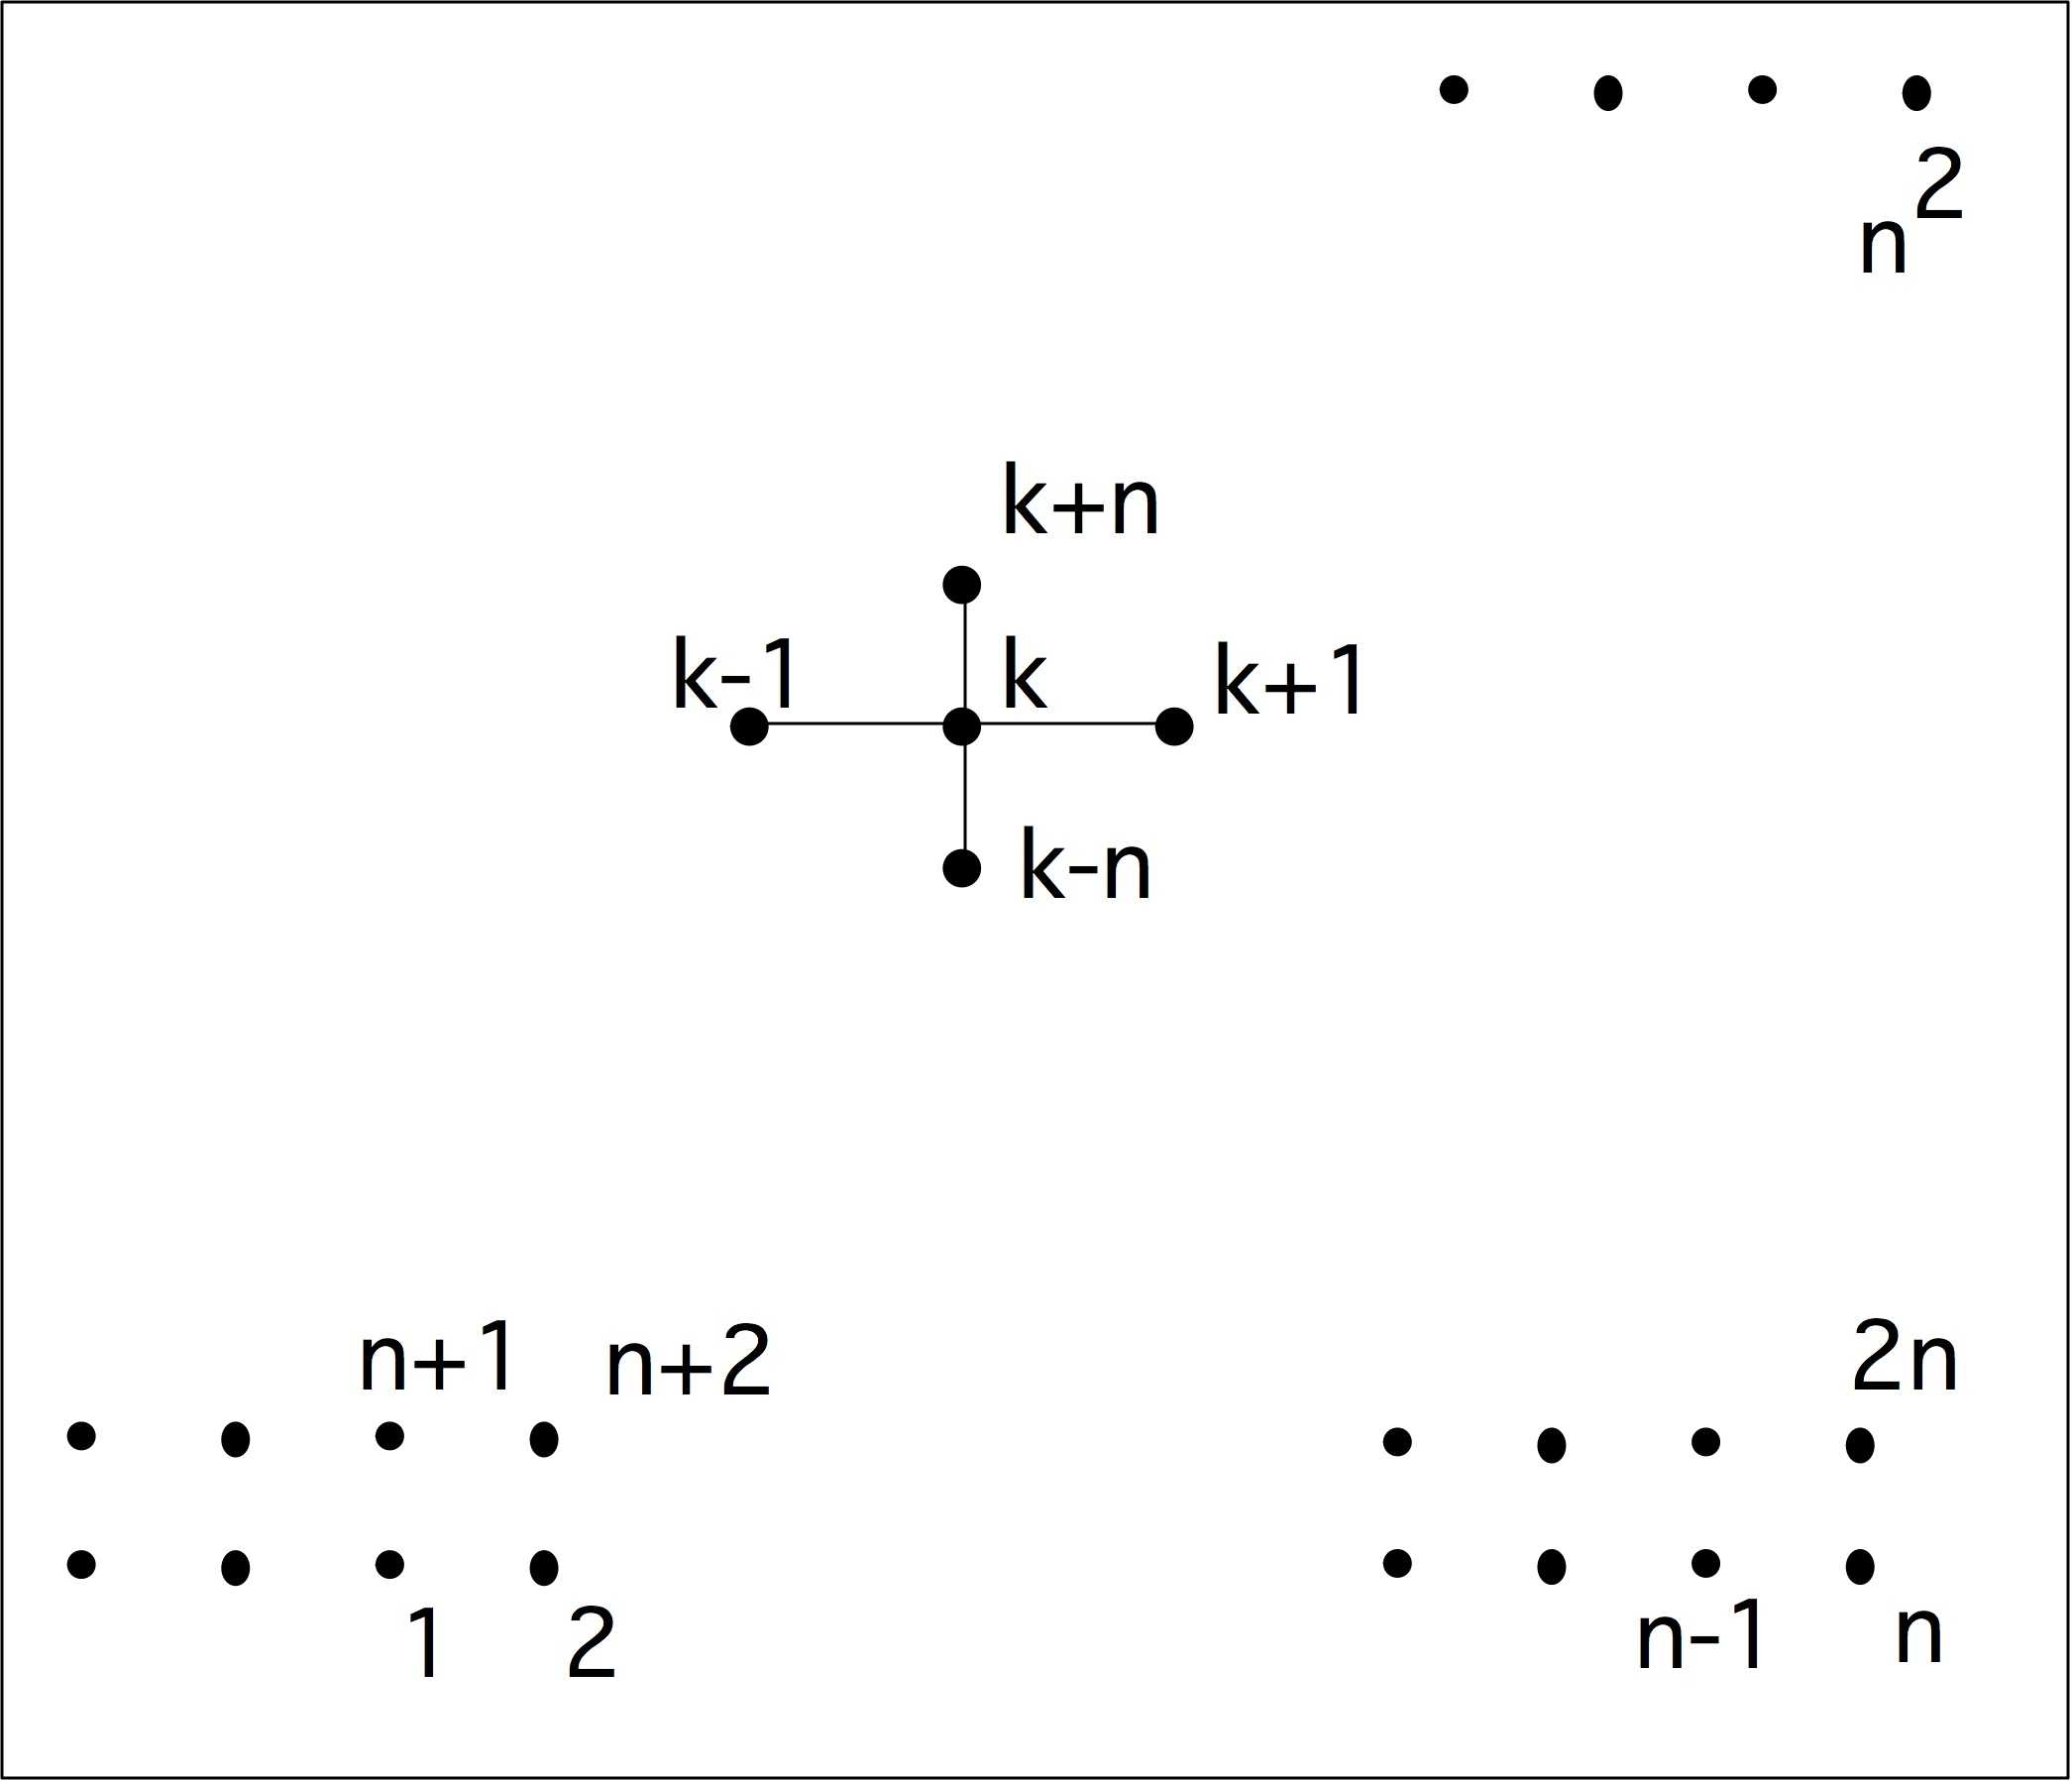
\includegraphics[scale=.07]{graphics/laplacedomain}
\hskip10pt\parbox{2in}{This is a graph!}}
}

\frame{\frametitle{The graph view of things}
Poisson eq:
\[ 4u_k-u_{k-1}-u_{k+1}-u_{k-n}-u_{k+n}=f_k \]
Consider a graph where $\{u_k\}_k$ are the edges\\
and $(u_i,u_j)$ is an edge iff $a_{ij}\not=0$.

This is the (adjacency) graph of a sparse matrix.
}

\frame{\frametitle{Sparse matrix from 2D equation}
\small
\[
  \left(\begin{array}{ccccc|ccccc|cc}
    4&-1&&&\emptyset&-1&&&&\emptyset&\\ 
    -1&4&1&&&&-1&&&&\\ 
    &\ddots&\ddots&\ddots&&&&\ddots&&\\ 
    &&\ddots&\ddots&-1&&&&\ddots&\\ 
    \emptyset&&&-1&4&\emptyset&&&&-1&\\ \hline
    -1&&&&\emptyset&4&-1&&&&-1\\
    &-1      &      &&&-1      &4       &-1      &&&&-1\\
    &\uparrow&\ddots&&&\uparrow&\uparrow&\uparrow&&  &&\uparrow\\
    &k-n     &      &&&k-1     &k       &k+1     &&-1&&k+n\\
    &&&&-1&&&&-1&4&&\\ \hline
    &        &      &&&\ddots  &        &        &&  &\ddots\\
  \end{array}\right)
\]
}


\frame{\frametitle{Matrix properties}

  \begin{itemize}
  \item Very sparse, banded
  \item Symmetric (only because 2nd order problem)
  \item Sign pattern: positive diagonal, nonpositive off-diagonal\\
    (true for many second order methods)
  \item Positive definite (just like the continuous problem)
  \item Constant diagonals: only because of the constant coefficient
    differential equation
  \end{itemize}
}

\frame{\frametitle{Realistic meshes}
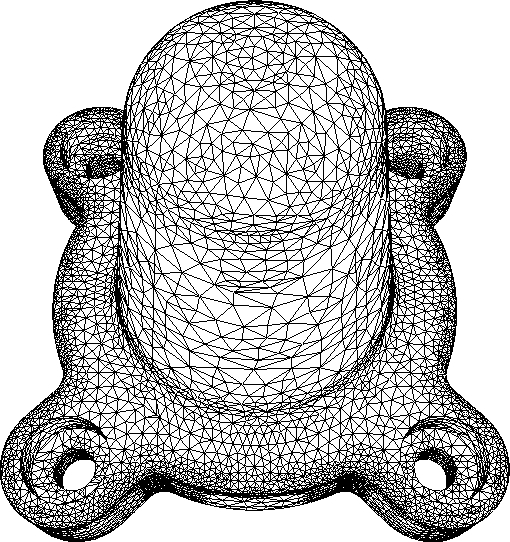
\includegraphics[scale=.3]{graphics/img206}
}

\frame{\frametitle{Sparse matrix storage}

 Matrix above has many zeros: $n^2$ elements but only $O(n)$
  nonzeros. Big waste of space to store this as square array.

 Matrix is called  `sparse' if there are enough zeros to make
  specialized storage feasible.

  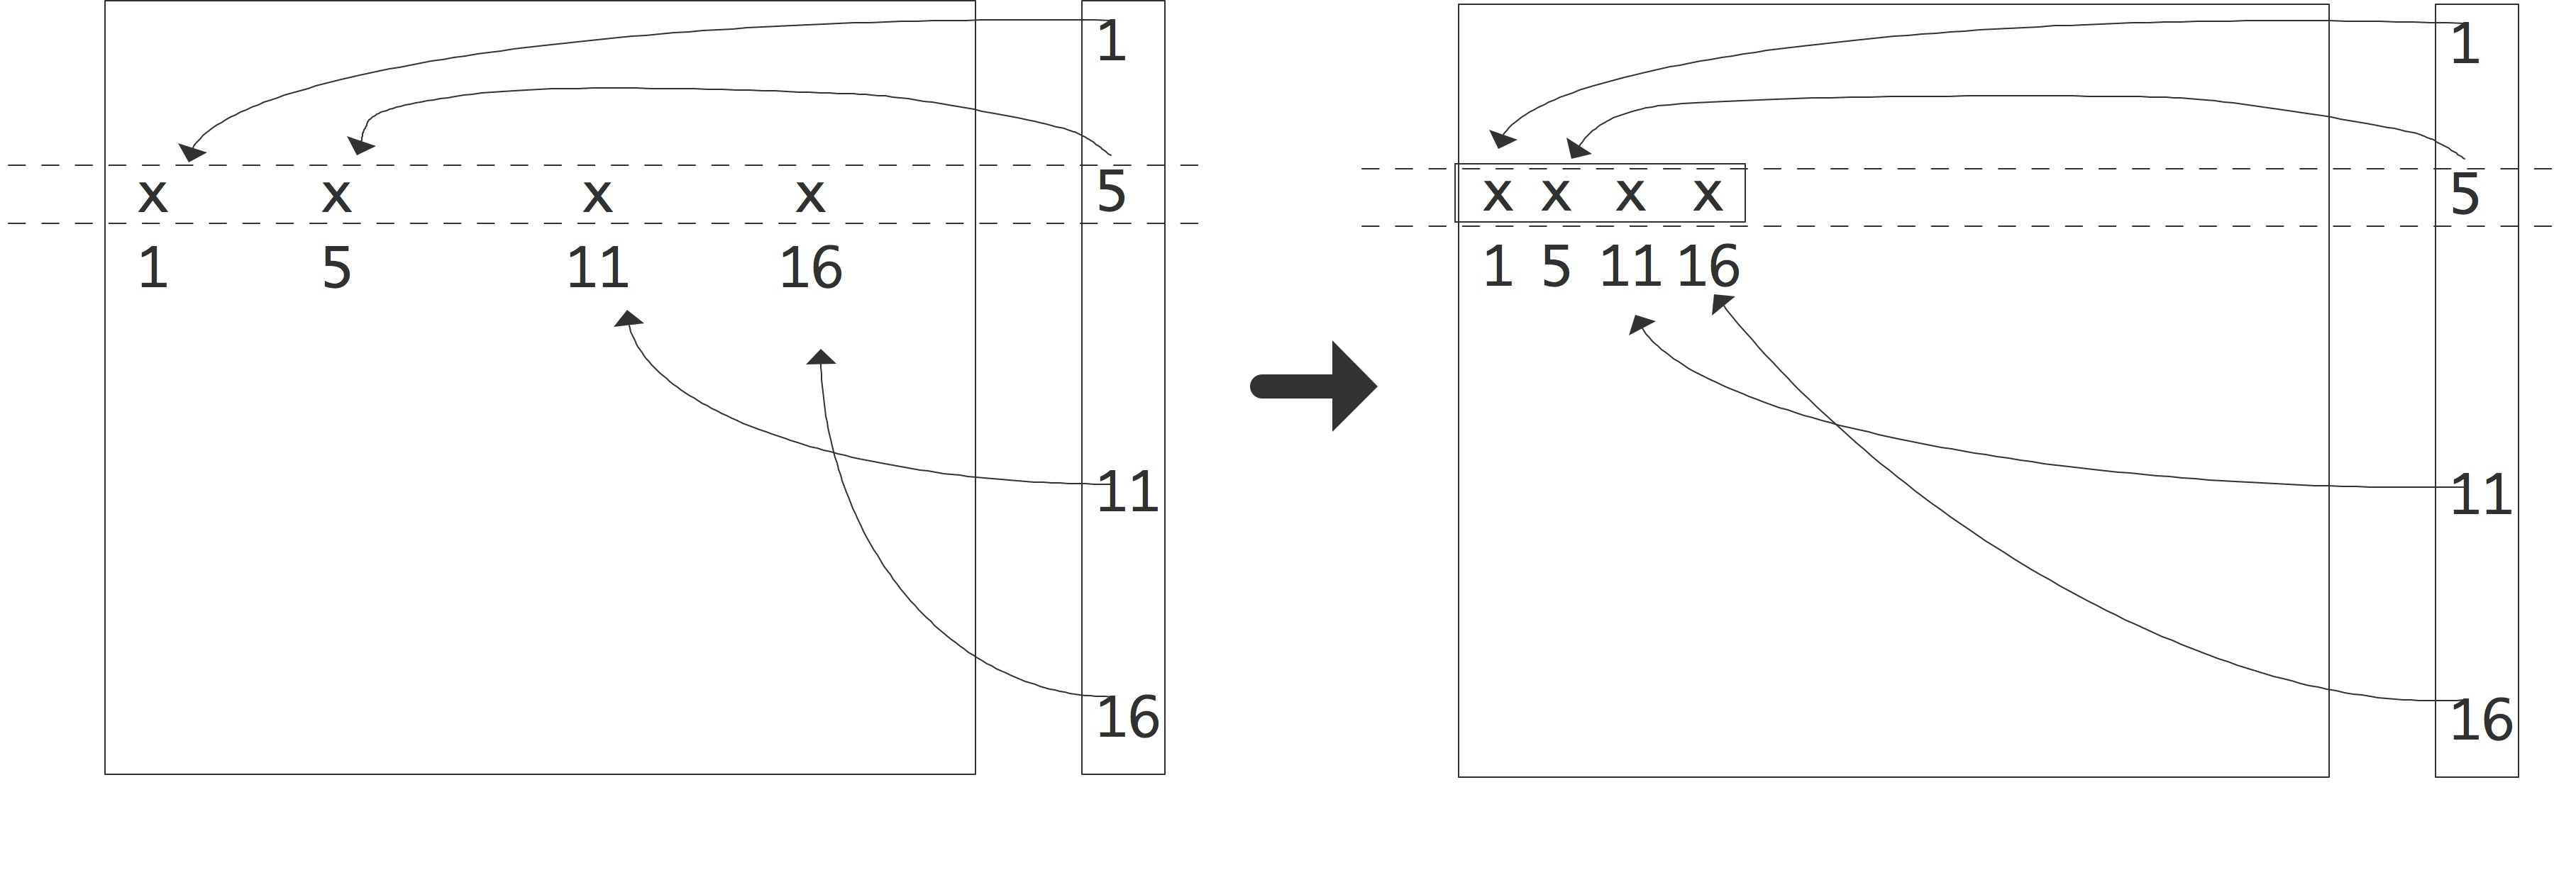
\includegraphics[scale=.08]{graphics/crs}
}

\frame{\frametitle{Compressed Row Storage}
\begin{equation}
A =
\left(\begin{array}{rrrrrr}
      10 &  0 &  0 & 0  &-2 &  0 \\
       3 &  9 &  0 & 0  & 0 &  3 \\
       0 &  7 &  8 & 7  & 0 &  0 \\
       3 &  0 &  8 & 7  & 5 &  0 \\
       0 &  8 &  0 & 9  & 9 & 13 \\
       0 &  4 &  0 & 0  & 2 & -1
           \end{array}
\right) ~.
\end{equation}
 Compressed Row Storage (CRS): store all nonzeros by row, their column
  indices, pointers to where the columns start (1-based indexing):
\begin{center}
\begin{tabular}{|r|r|r|r|r|r|r|r|r|r|r|r|r|r|r|r|} \hline
{\tt val}     &10 &-2& 3& 9& 3& 7& 8& 7& 3 $\cdots$  9&13& 4& 2&-1 \\ \hline
{\tt col\_ind}& 1 & 5& 1& 2& 6& 2& 3& 4& 1 $\cdots$  5& 6& 2& 5& 6 \\ \hline
\end{tabular} \\
\vspace{.02 in}
\begin{tabular}{|r|r|r|r|r|r|r|r|} \hline
{\tt row\_ptr}& 1 & 3 & 6 & 9 & 13 & 17 & 20  \\ \hline
\end{tabular} ~.
\end{center}
}

% \frame{\frametitle{Band matrix storage}

%  Matrix from 5-point stencil is a band matrix:
% \[ \exists_{p,q\geq0}\colon (j<i-p\vee j>i+q)\rightarrow a_{ij}=0 \]
% }

\frame[containsverbatim]{\frametitle{Sparse matrix operations}

  Most common operation: matrix-vector product
\begin{verbatim}
for (row=0; row<nrows; row++) {
   s = 0;
   for (icol=ptr[row]; icol<ptr[row+1]; icol++) {
      int col = ind[icol];
      s += a[aptr] * x[col];
      aptr++;
   }
   y[row] = s;
}
\end{verbatim}
Operations with changes to the nonzero structure are much harder!

Indirect addressing of \texttt{x} gives low spatial and temporal locality.
}

\frame{\frametitle{Graph theory of sparse matrices}
  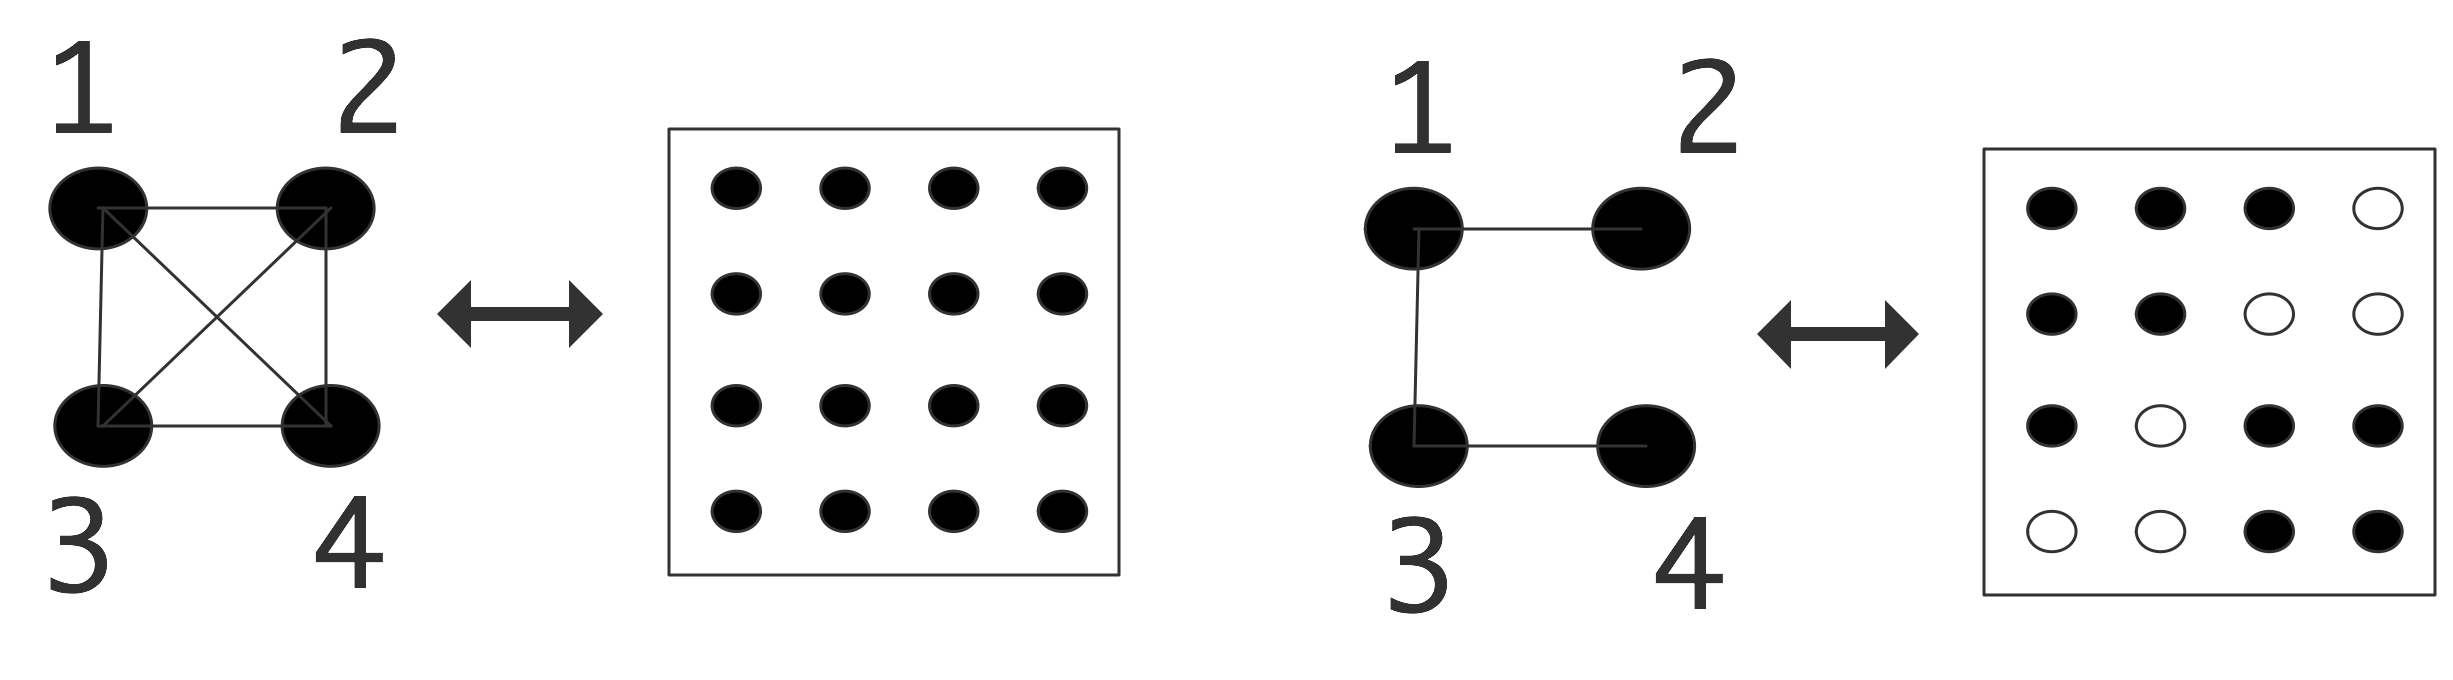
\includegraphics[scale=.12]{graphics/matrix-graph}
}

\frame{\frametitle{Graph theory of sparse elimination}
  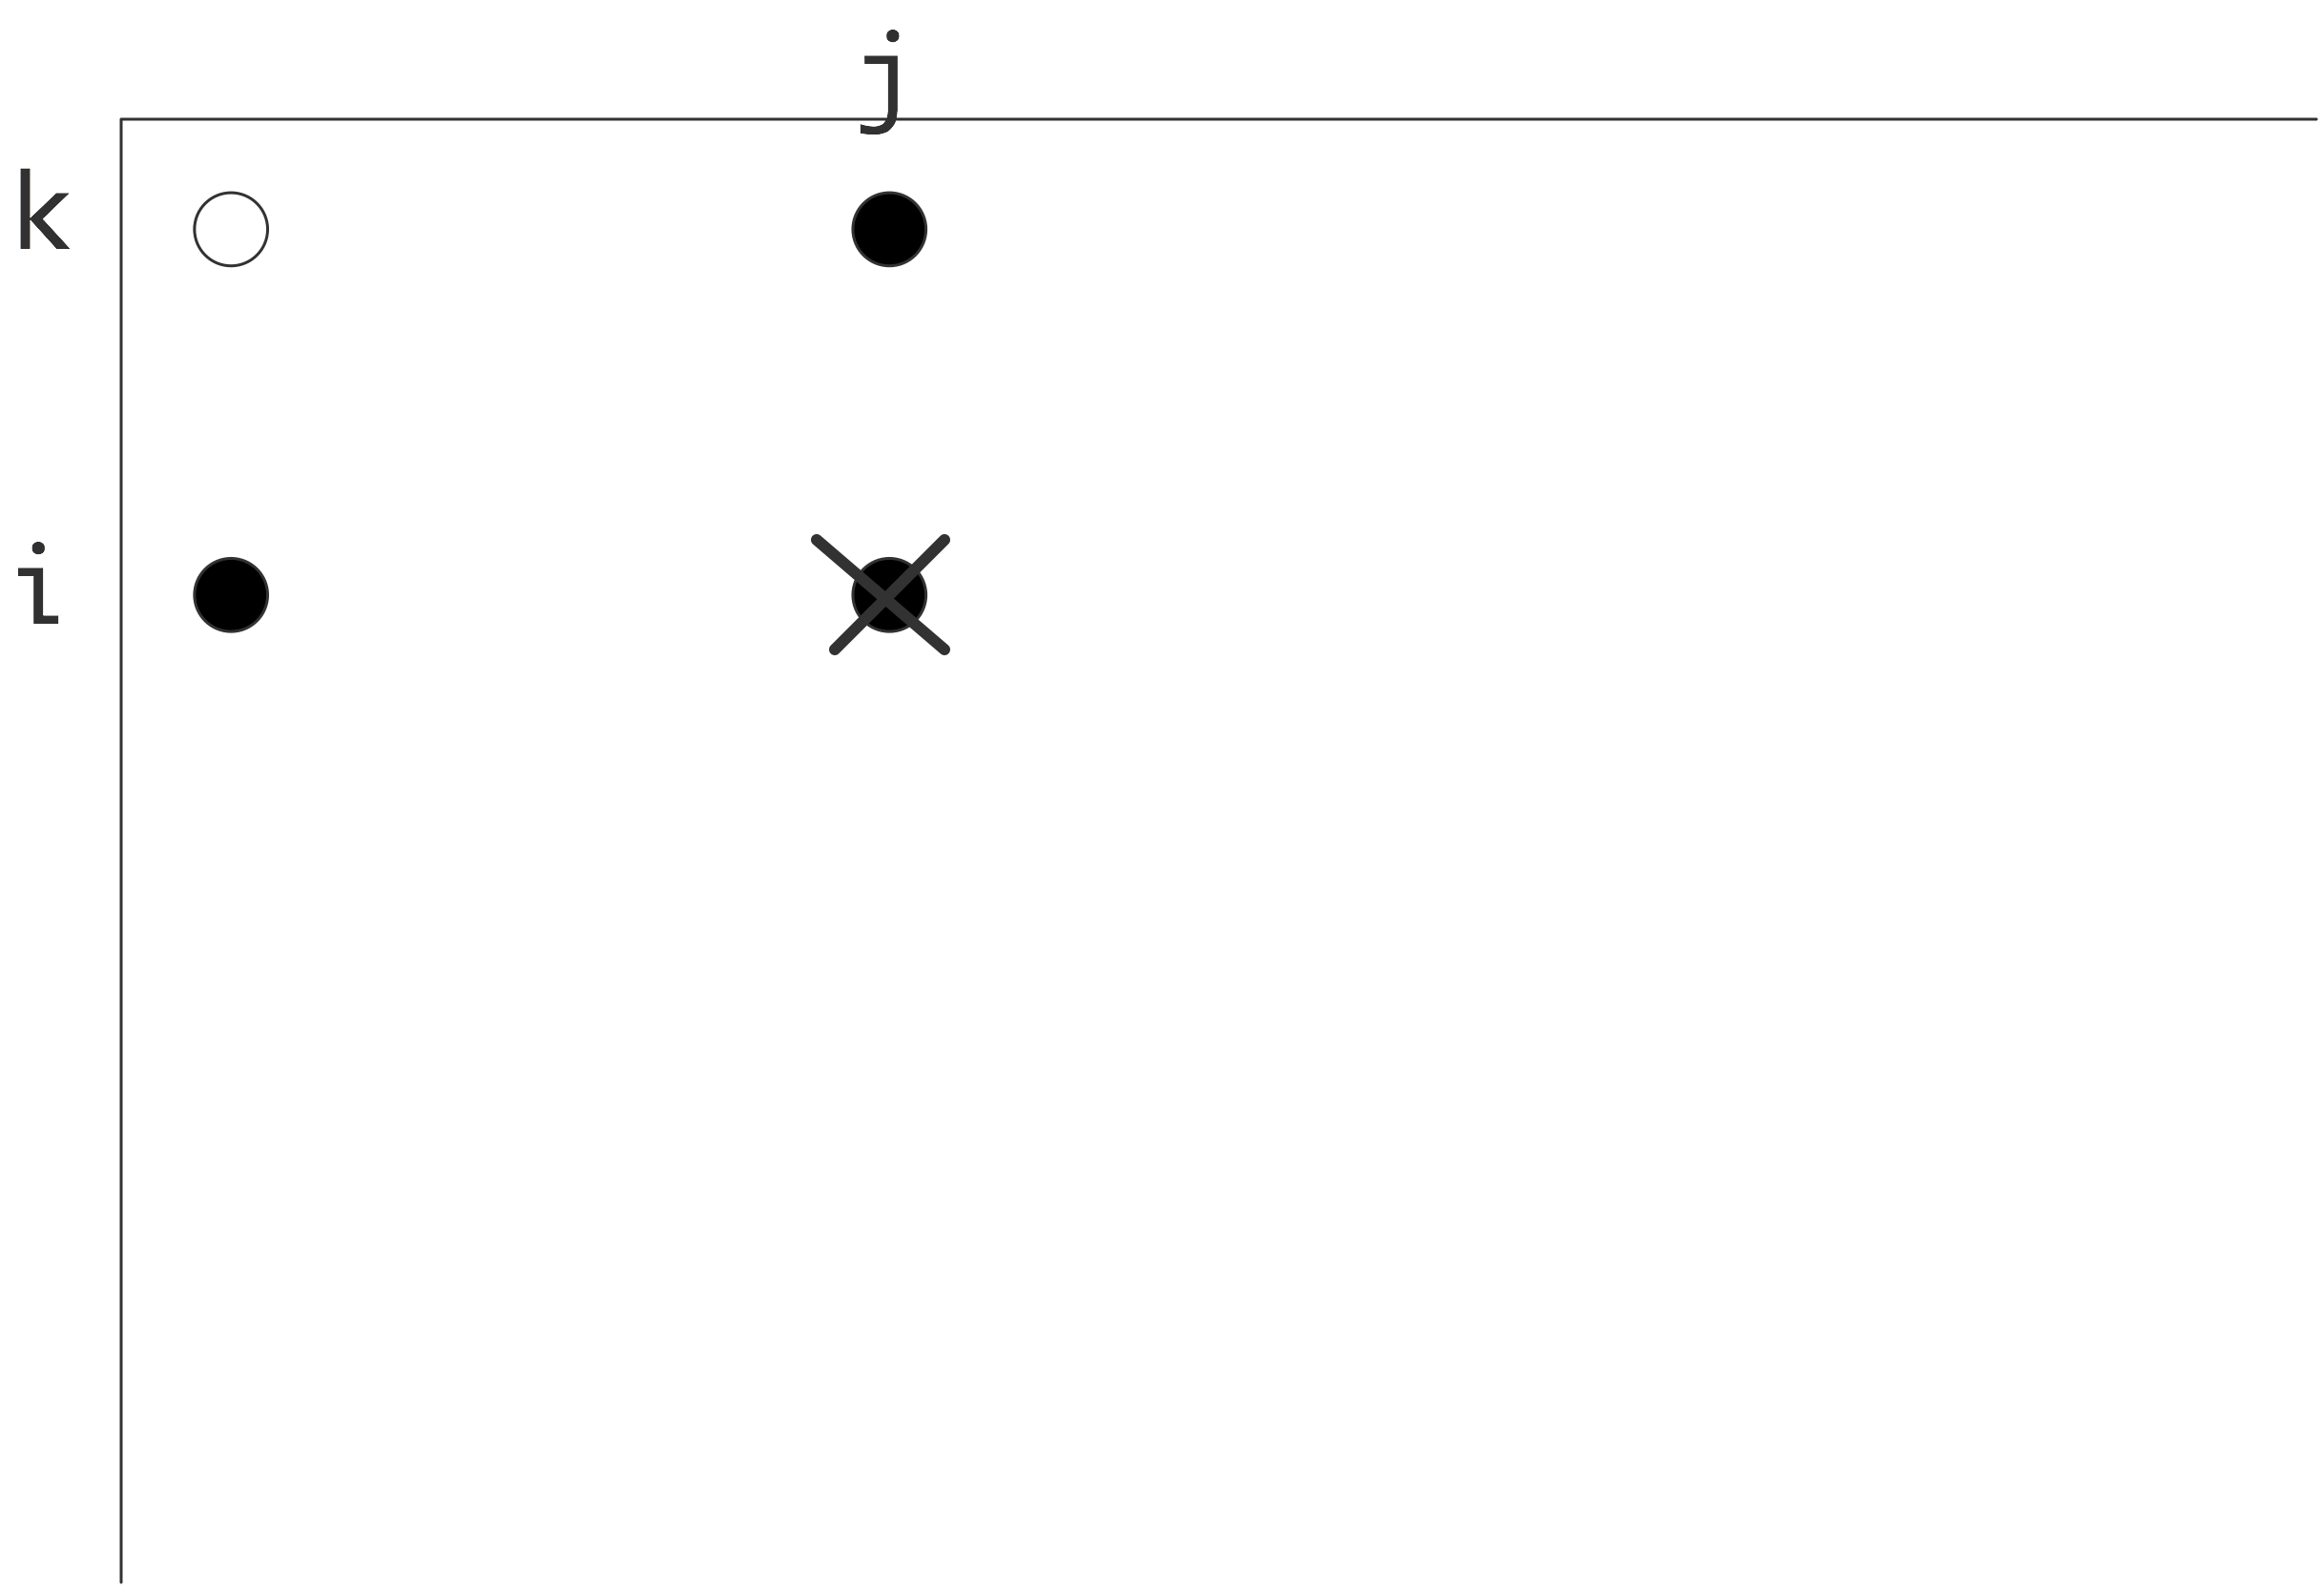
\includegraphics[scale=.06]{graphics/ijk-matrix-eliminate}
$a_{ij} \leftarrow a_{ij}- a_{ik}a_{kk}\inv a_{kj}$

  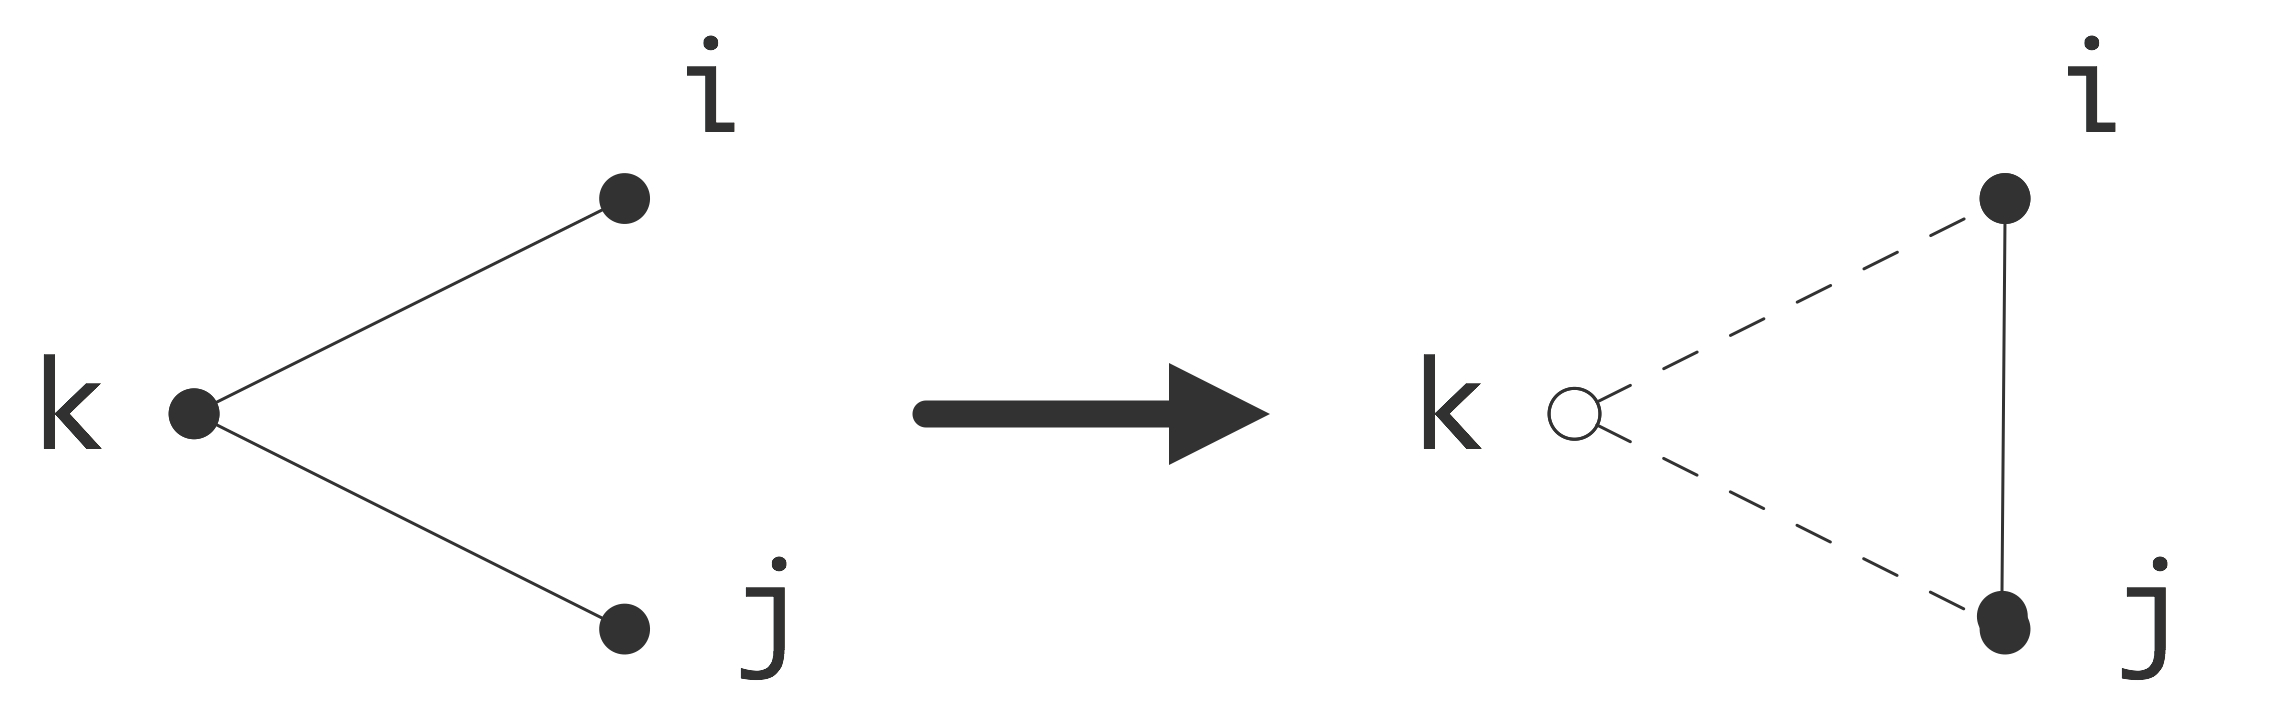
\includegraphics[scale=.1]{graphics/ijk-eliminate}
}

\frame{\frametitle{Fill-in}
Fill-in: index $(i,j)$ where $a_{ij}=0$ but $\ell_{ij}\not=0$ or
$u_{ij}\not=0$.
}

\frame{\frametitle{Fill-in is a function of ordering}
  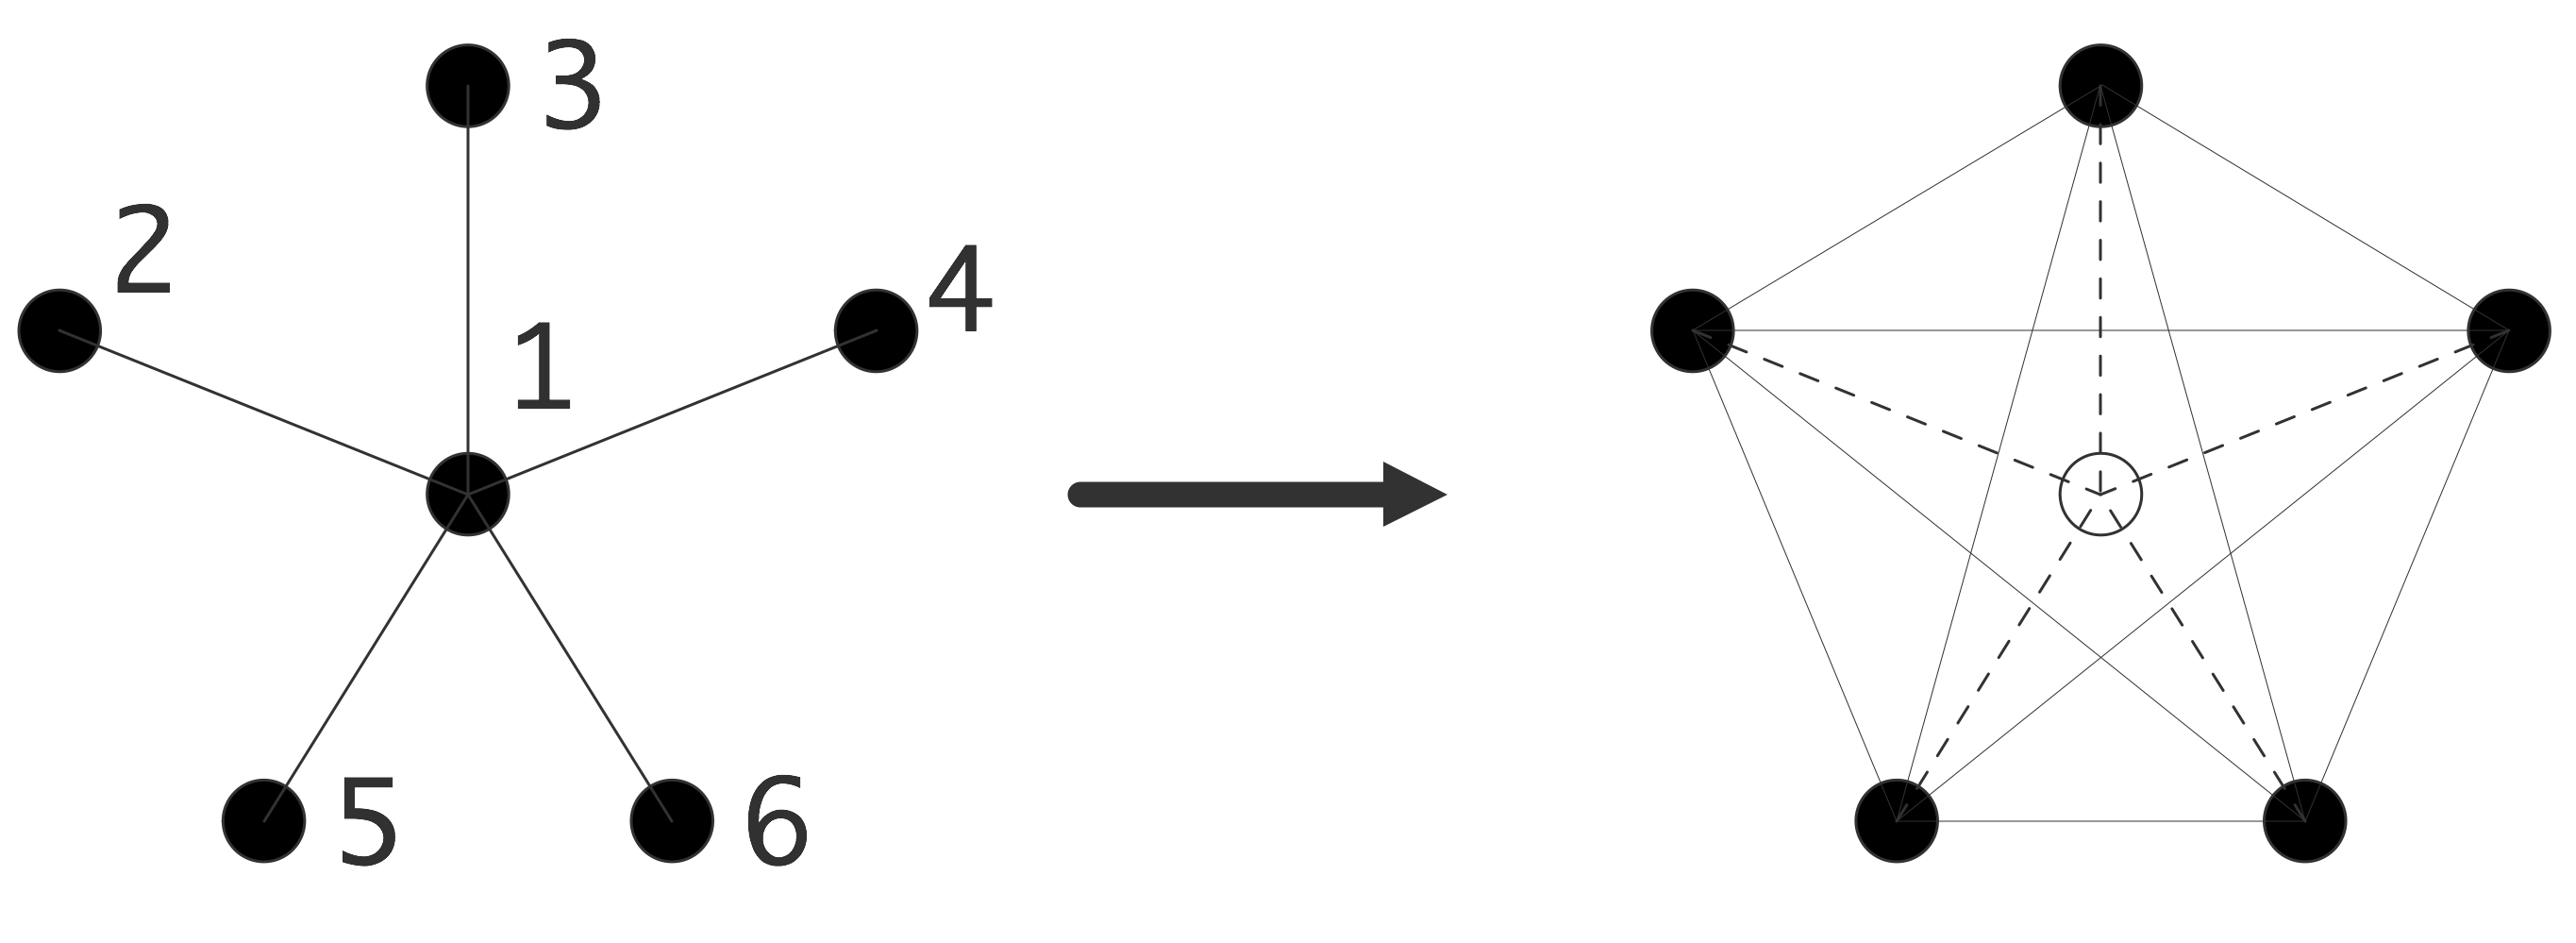
\includegraphics[scale=.1]{graphics/starmatrix}
  \[ 
  \begin{pmatrix}
    *&*&\cdots&*\\ *&*&&\emptyset\\ \vdots&&\ddots\\ *&\emptyset&&*
  \end{pmatrix}
  \]
  After factorization the matrix is dense.\\
  Can this be permuted?
}

\frame{\frametitle{LU of a sparse matrix}
\small
\[
\left(\begin{array}{ccccc:cccc}
  4&-1&0&\ldots&&-1\\ -1&4&-1&0&\ldots&0&-1\\ 
  &\ddots&\ddots&\ddots&&&\ddots\\ \hdashline
  -1&0&\ldots&&&4&-1\\ 0&-1&0&\ldots&&-1&4&-1\\
\end{array}\right)
\] \[
\Rightarrow\quad
\left(\begin{array}{c|cccc:cccc}
  4&-1&0&\ldots&&-1\\ \hline &4-\frac14&-1&0&\ldots&-1/4&-1\\ 
  &\ddots&\ddots&\ddots&&&\ddots\\ \hdashline
  &-1/4&\ldots&&&4-\frac14&-1\\ &-1&0&\ldots&&-1&4&-1\\
\end{array}\right)
\]
}

\frame{
  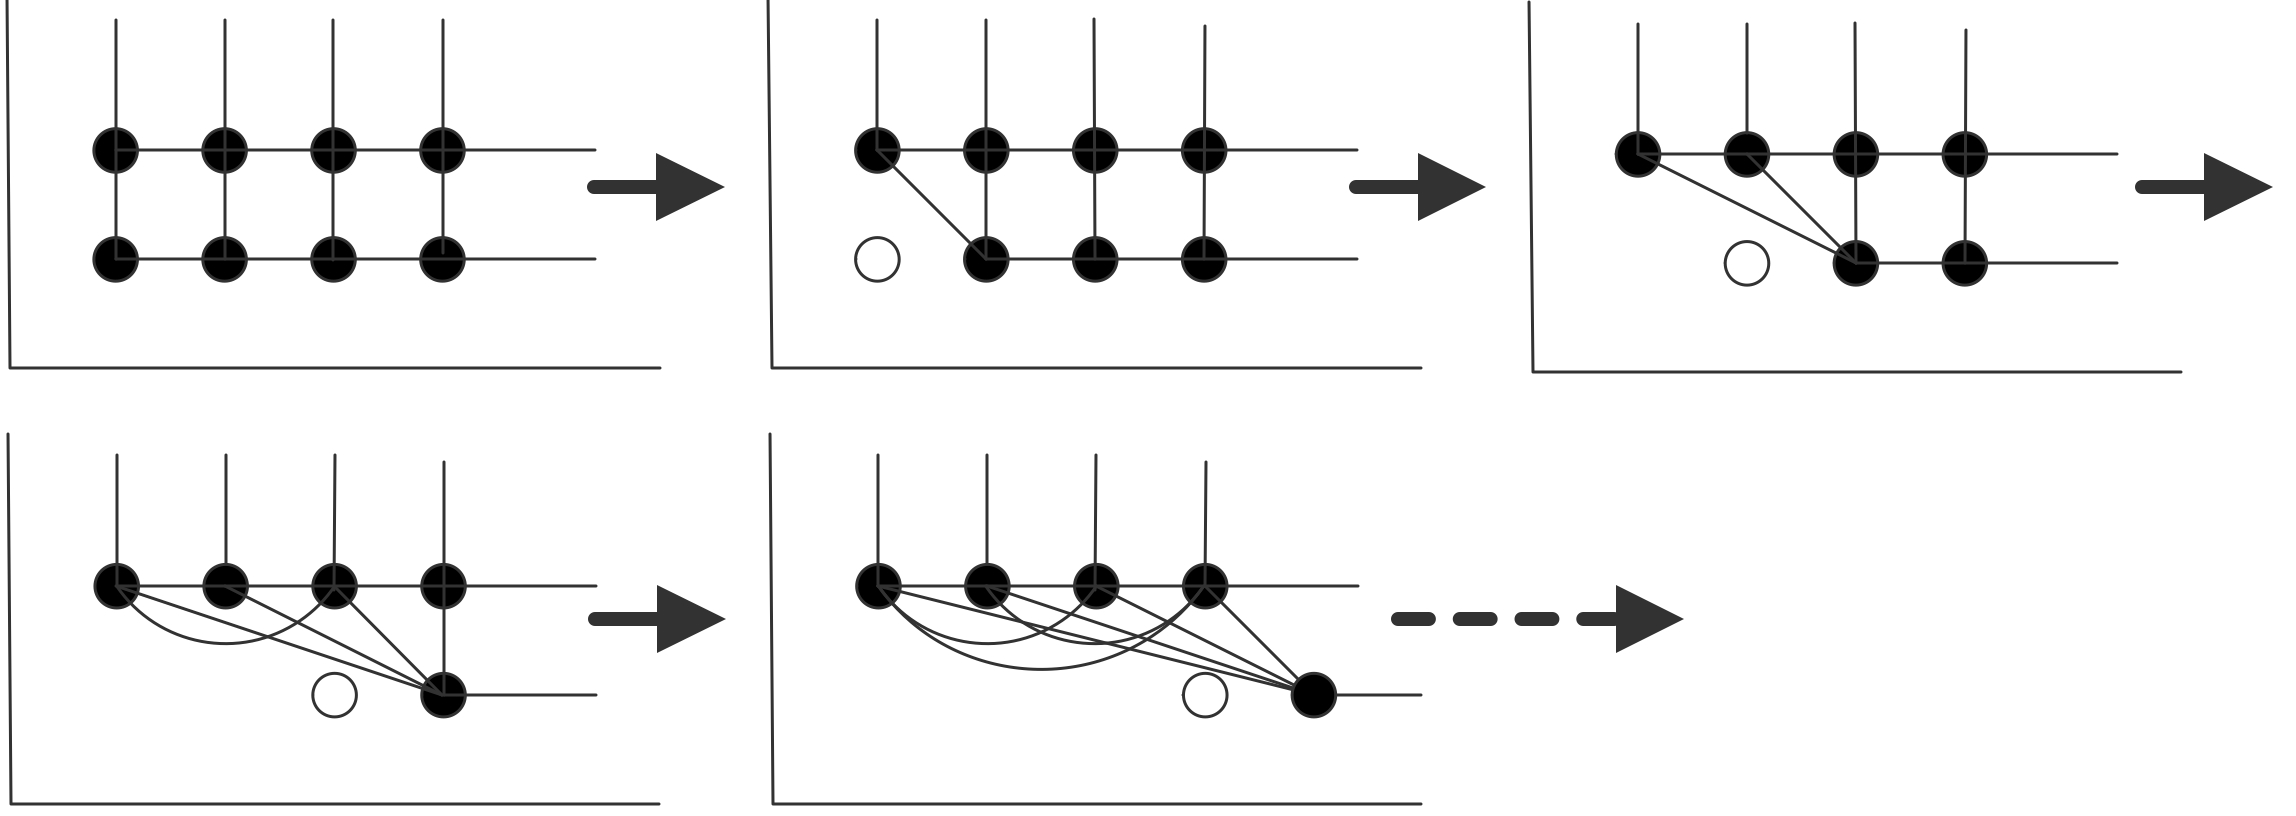
\includegraphics[scale=.15]{graphics/row-eliminate}

Remaining matrix has a dense leading block
}

\frame{\frametitle{Fill-in during LU}

2D BVP: $\Omega$ is $n\times n$, gives matrix of size $N=n^2$, with
bandwidth~$n$. 

Matrix storage $O(N)$

LU storage $O(N^{3/2})$

LU factorization work $O(N^2)$

Cute fact: storage can be computed linear in \#nonzeros
}

\end{document}

\frame{\frametitle{Fill-in is a function of ordering}

  \[ 
  \begin{pmatrix}
    *&*&\cdots&*\\ *&*&&\emptyset\\ \vdots&&\ddots\\ *&\emptyset&&*
  \end{pmatrix}
  \]
  After factorization the matrix is dense.\\
  Can this be permuted?
}

\frame{\frametitle{Domain decomposition}
    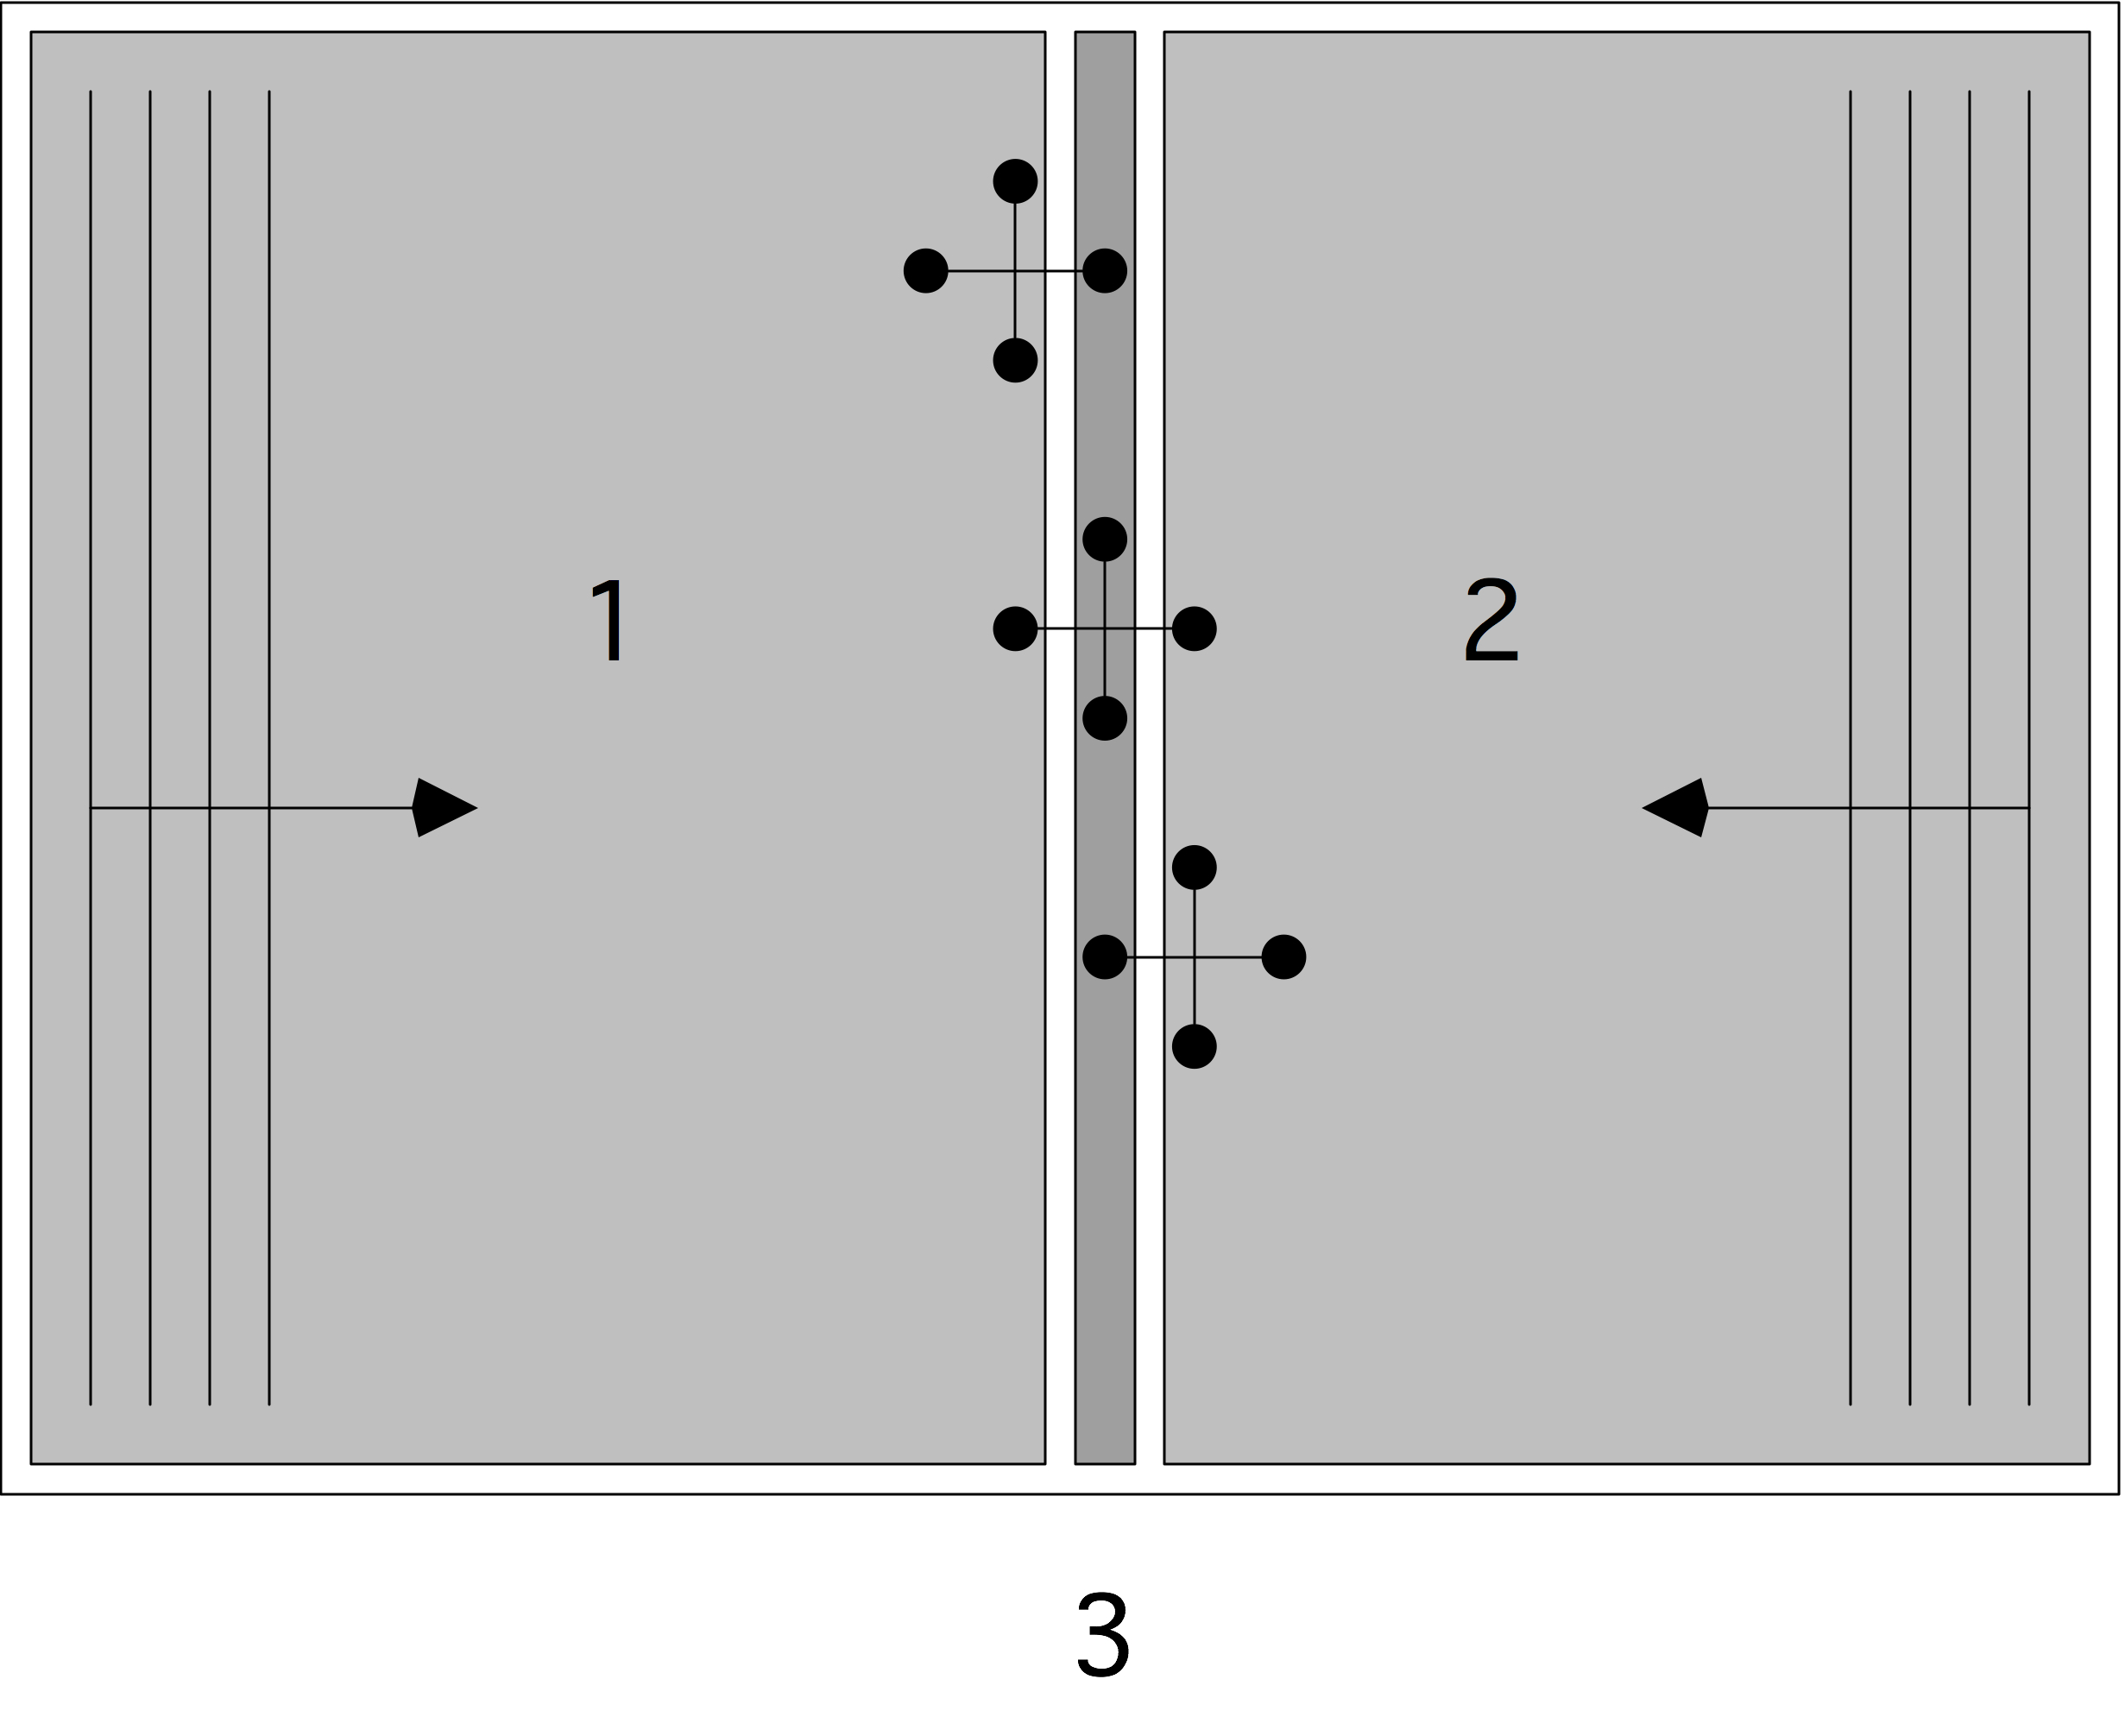
\includegraphics[scale=.1]{graphics/domdecomp}
}

\newcommand\Add{A^{\mathrm{DD}}}

\frame{\small
\[
\left(\begin{array}{ccccc|ccccc|c}
  \star&\star &      &      &      &&&&&&0\\
  \star&\star &\star &      &      &&&&&&\vdots\\
       &\ddots&\ddots&\ddots&      &&&\emptyset&&&\vdots\\
       &      &\star &\star &\star &&&&&&0\\
       &      &      &\star &\star &&&&&&\star\\ \hline
  &&&&&\star&\star &      &      &      &0\\
  &&&&&\star&\star &\star &      &      &\vdots\\
  &&\emptyset&&&     &\ddots&\ddots&\ddots&      &\vdots\\
  &&&&&     &      &\star &\star &\star &0\\
  &&&&&     &      &      &\star &\star &\star\\ \hline
  0&\cdots&\cdots&0&\star&0&\cdots&\cdots&0&\star&\star
\end{array}\right)
\begin{array}{c}
  \left.\begin{array}{c}
    \phantom{x}\\ \phantom{x}\\ \phantom{x}\\ \phantom{x}\\ \phantom{x}\\
  \end{array}\right\} \\
  \left.\begin{array}{c}
    \phantom{x}\\ \phantom{x}\\ \phantom{x}\\ \phantom{x}\\ \phantom{x}\\
  \end{array}\right\} \\
  \left.\begin{array}{c}
    \phantom{x}\\ 
  \end{array}\right\}
\end{array}
\begin{array}{c}
  \phantom{x}\\ \phantom{x}\\ (n^2-n)/2\\ \phantom{x}\\ \phantom{x}\\
  \phantom{x}\\ \phantom{x}\\ (n^2-n)/2\\ \phantom{x}\\ \phantom{x}\\
  n
\end{array}
\]
}

\frame{\frametitle{DD factorization}

\[
\begin{array}{l}
\Add=
  \begin{pmatrix}
    A_{11}&\emptyset&A_{13}\\
    \emptyset&A_{22}&A_{23}\\
    A_{31}&A_{32}&A_{33}
  \end{pmatrix}=\\[10pt]
  \begin{pmatrix}
    I\\
    \emptyset&I\\
    A_{31}A_{11}\inv&A_{32}A_{22}\inv&I
  \end{pmatrix}
  \begin{pmatrix}
    A_{11}&\emptyset&A_{13}\\
         &A_{22}&A_{23}\\
    &&S
  \end{pmatrix}
\end{array}
\]
\[ S = A_{33}-A_{31}A_{11}\inv A_{13}-A_{32}A_{22}\inv A_{23} \]
Parallelism\ldots
}

\frame{\frametitle{Graph theory of sparse elimination}
\only<1,3>{
\[ a_{ij} \leftarrow a_{ij}- a_{ik}a_{kk}\inv a_{kj} \]
  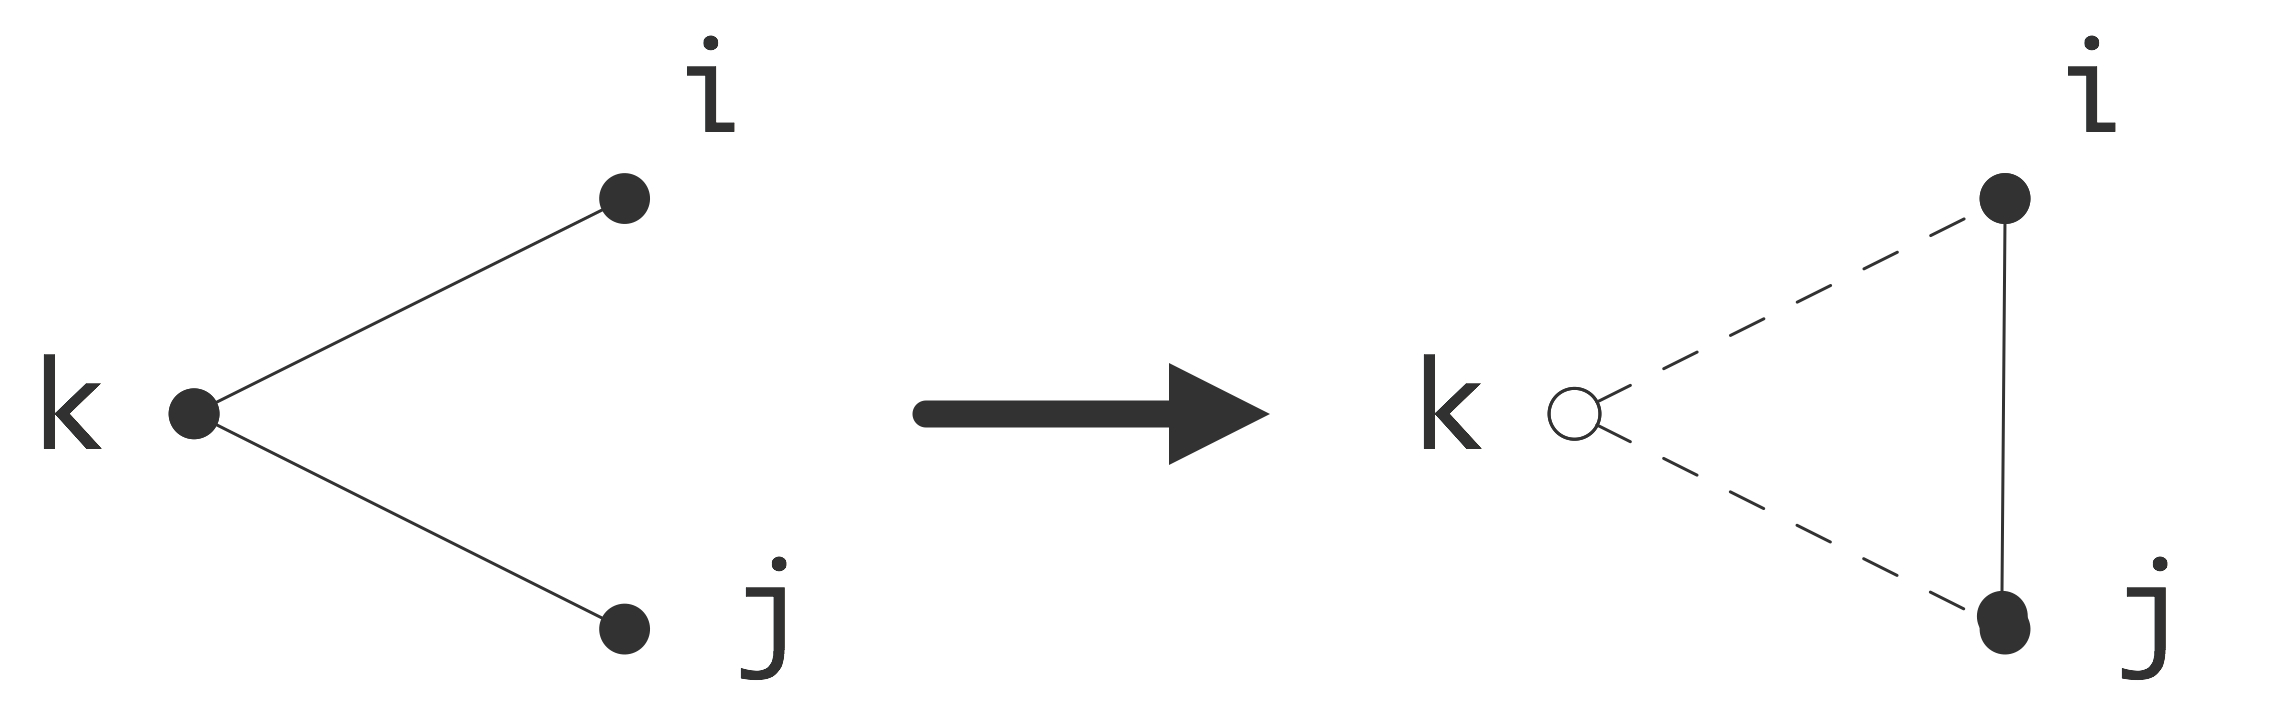
\includegraphics[scale=.12]{graphics/ijk-eliminate}
}

\only<2>{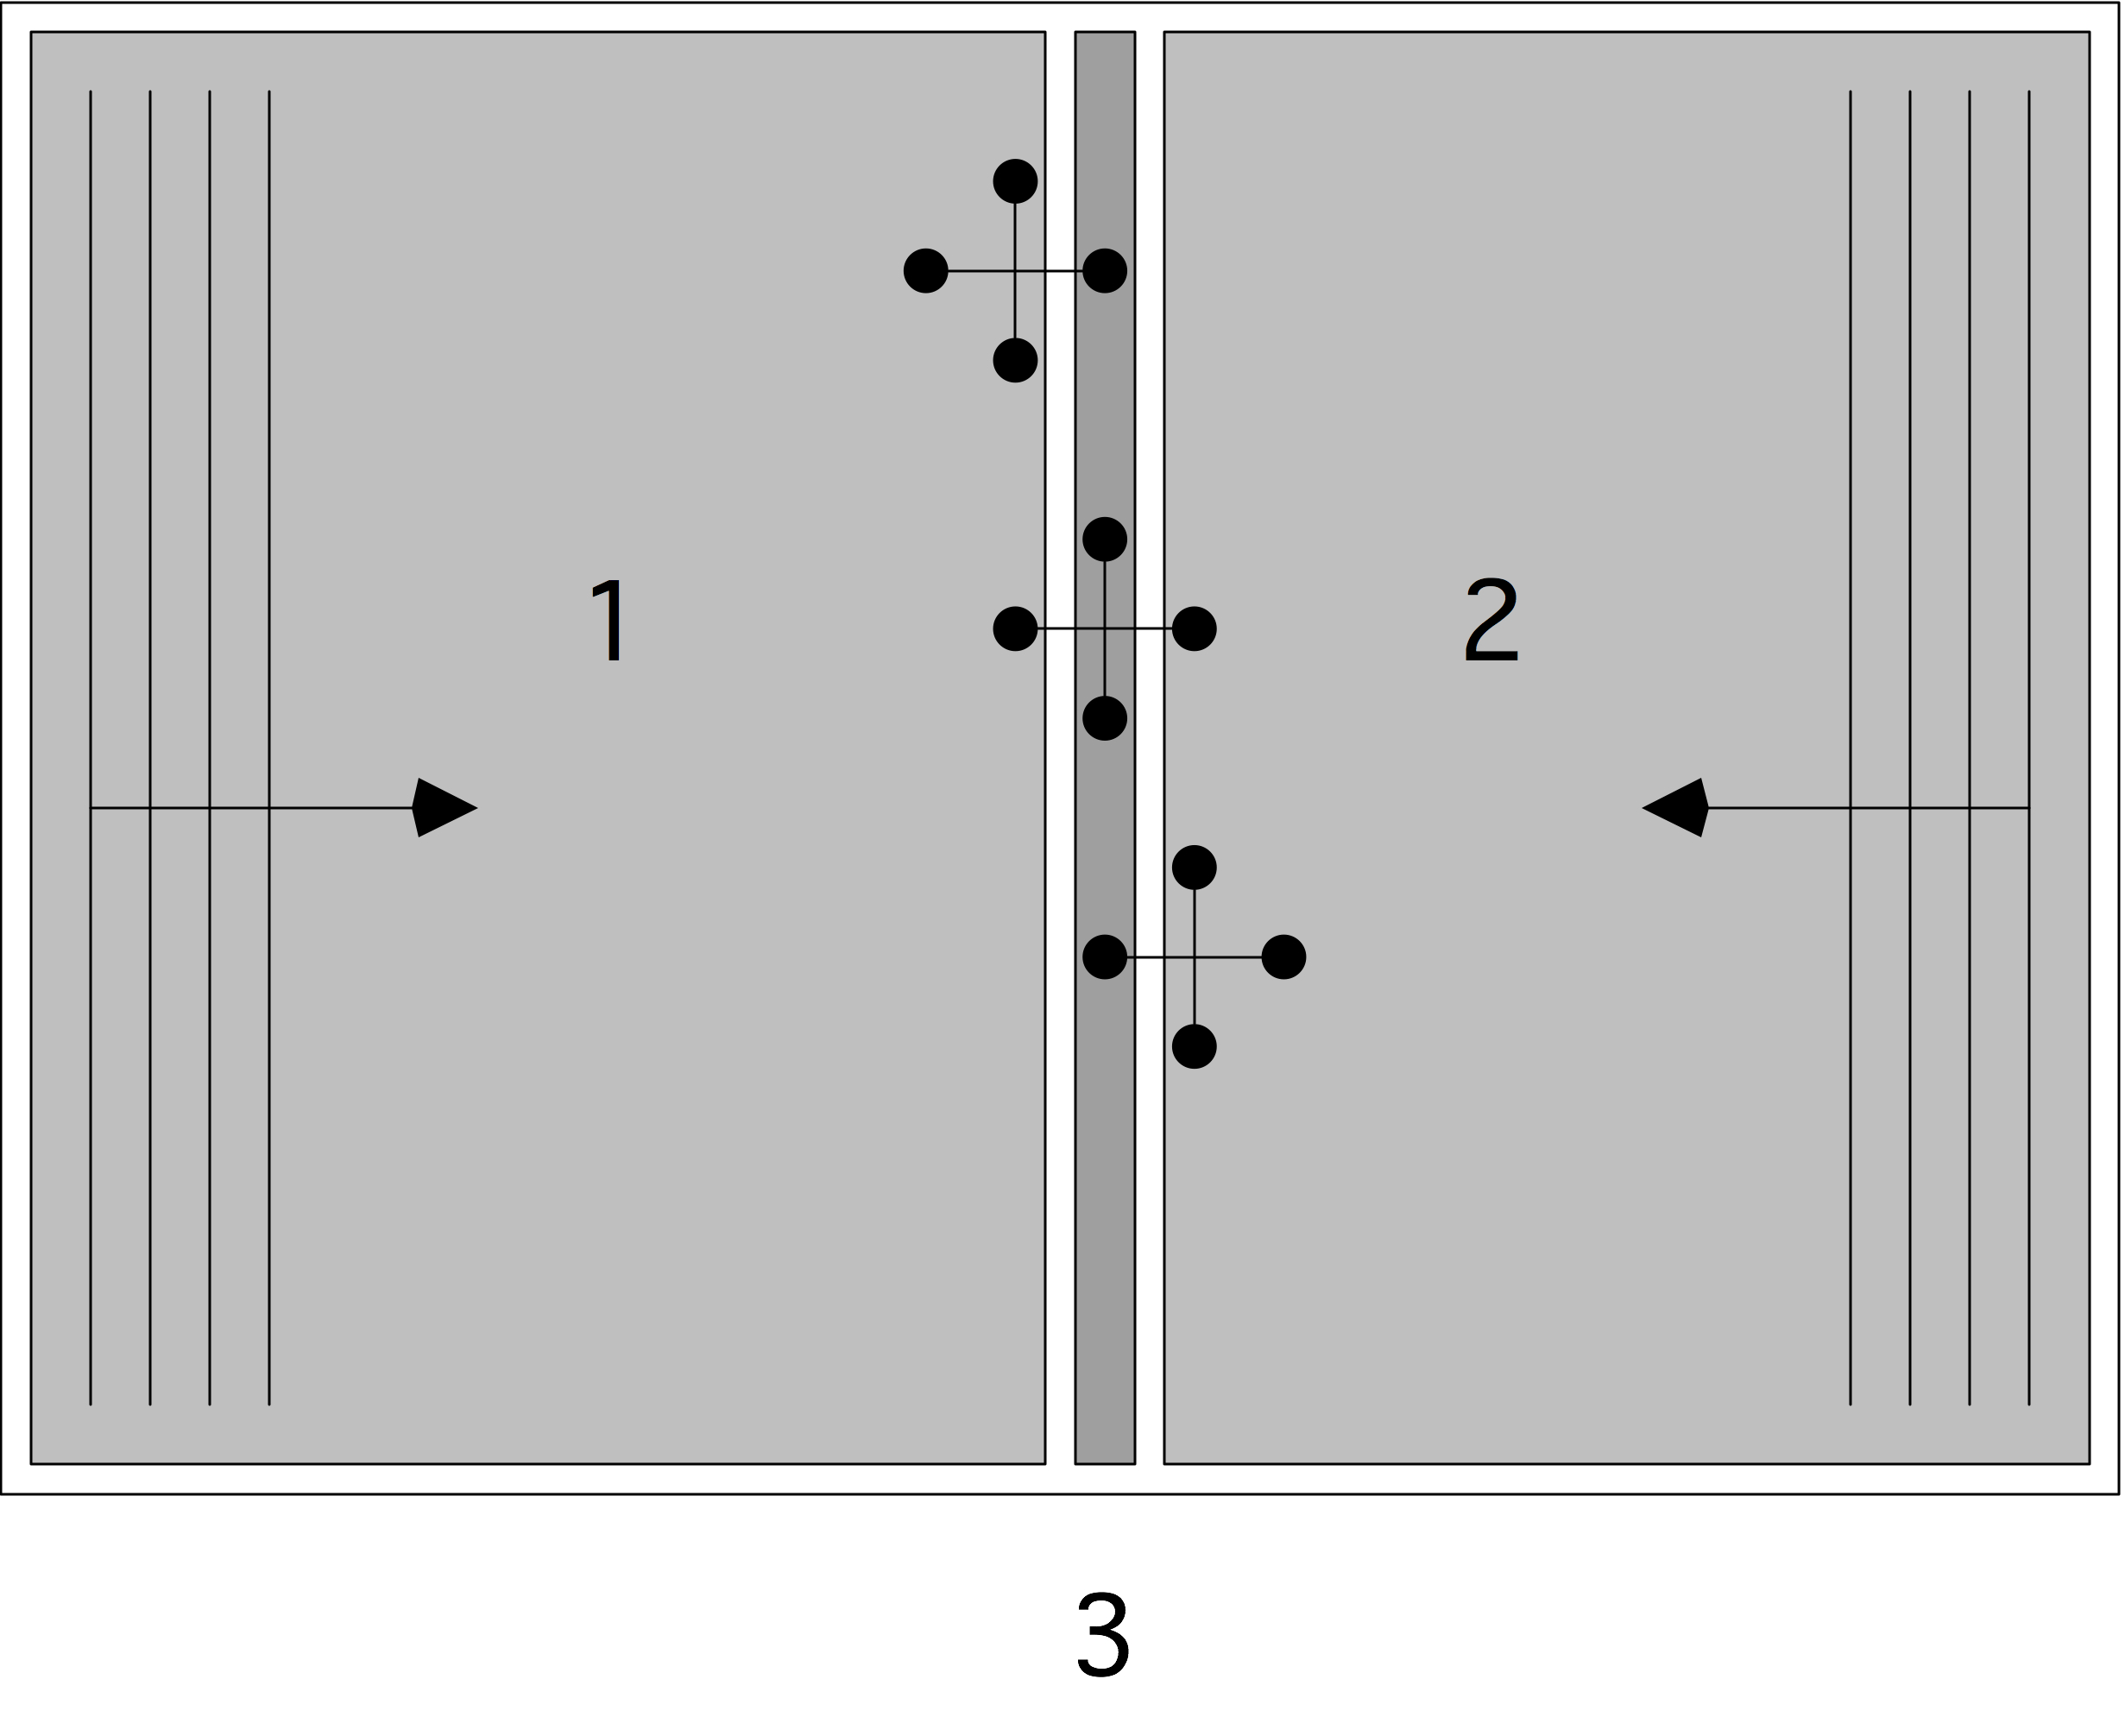
\includegraphics[scale=.08]{graphics/domdecomp}}

\only<3->{So inductively $S$ is dense}
}

\frame{\frametitle{Recursive bisection}
\begin{figure}
  \begin{quote}
    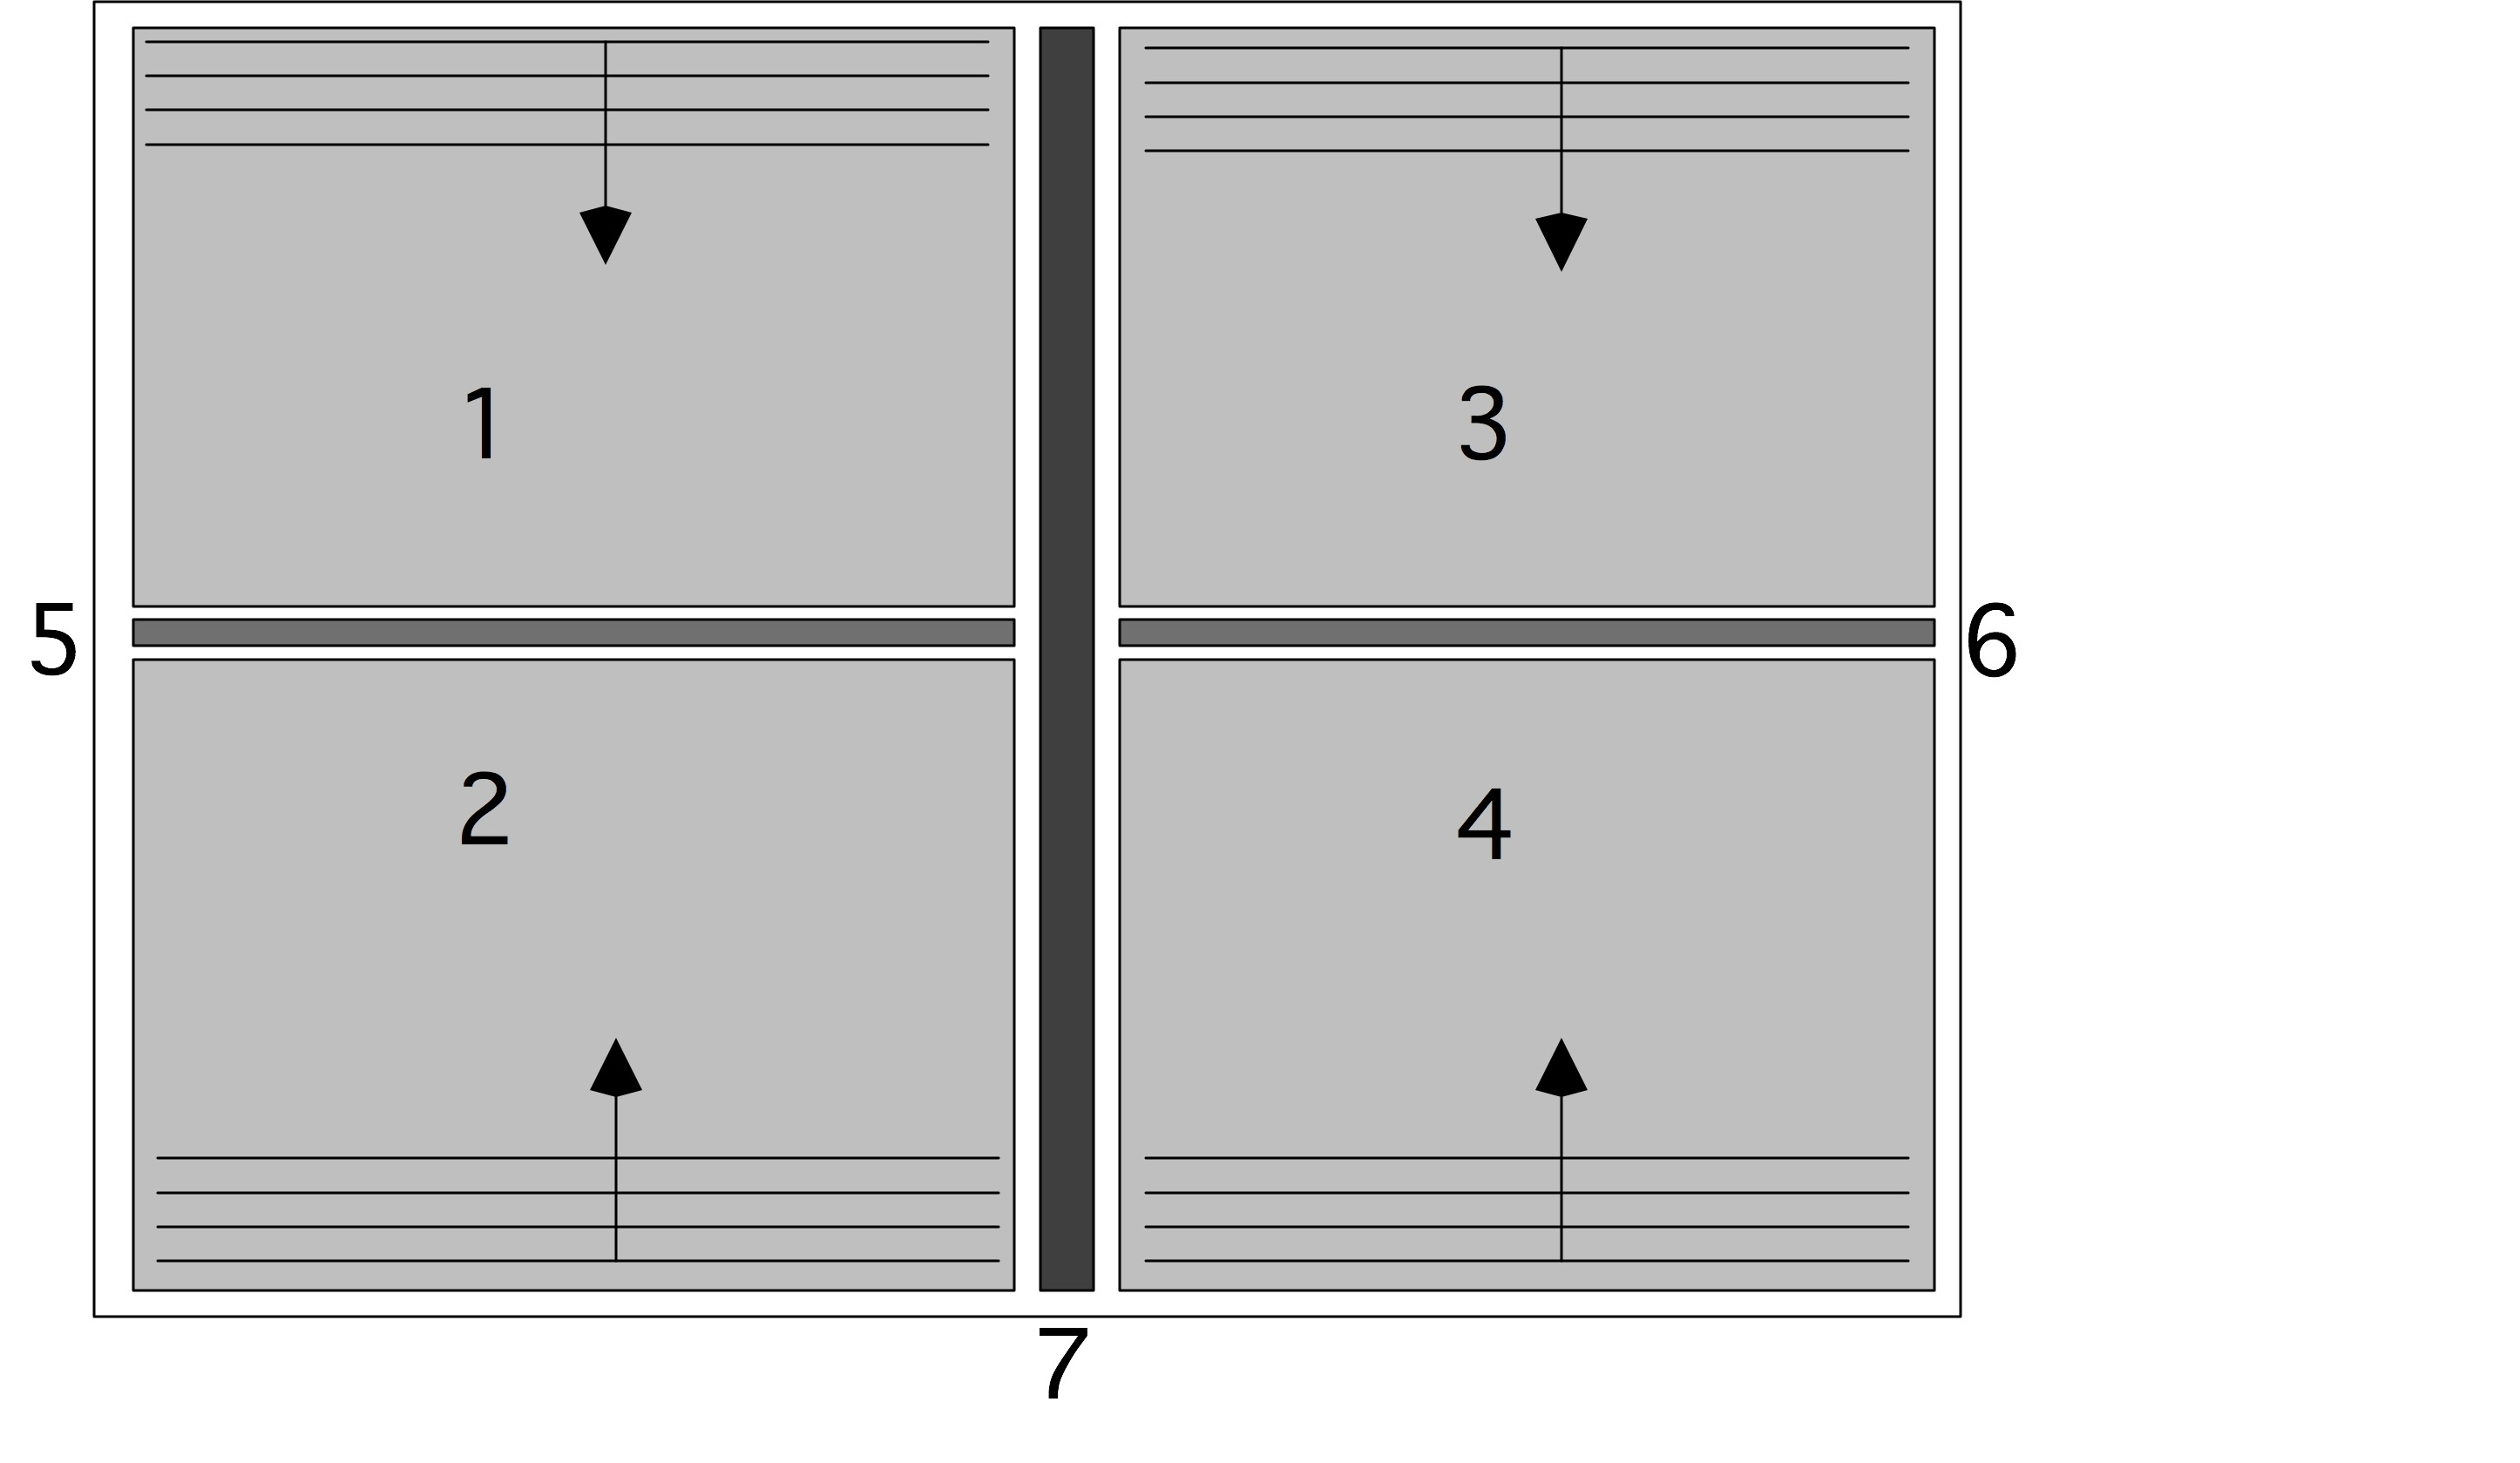
\includegraphics[scale=.11]{graphics/domdecomp2}
  \end{quote}
  \caption{A four-way domain decomposition}
  \label{fig:domdecomp2}
\end{figure}
}
\frame{
\[
  \Add=
  \left(\begin{array}{ccccccc}
    A_{11}&     &     &     &A_{15}&     &A_{17}\\
         &A_{22}&     &     &A_{25}&     &A_{27}\\
         &     &A_{33}&     &     &A_{36}&A_{37}\\
         &     &     &A_{44}&     &A_{46}&A_{47}\\ 
    A_{51}&A_{52}&    &     &A_{55}&      &A_{57}\\
         &      &A_{63}&A_{64}&    &A_{66}&A_{67}\\
    A_{71}&A_{72}&A_{73}&A_{74}&A_{75}&A_{76}&A_{77}
  \end{array}\right)
\]
The domain/operator/graph view is more insightful, don't you think?
}

\frame{\frametitle{How does this look in reality?}
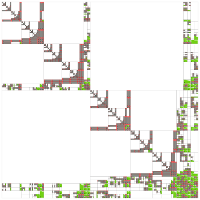
\includegraphics[scale=2.5]{graphics/nesteddis}
}

\frame{\frametitle{Complexity}
With $n=\sqrt N$:
\begin{itemize}
\item one dense matrix on a separator of size~$n$, plus
\item two dense matrices on separators of size~$n/2$
\item $\rightarrow 3/2\,n^2$ space and $5/12\,n^3$ time
\item and then four times the above with $n\rightarrow n/2$
\end{itemize}
\[ 
\begin{array}{r@{{}={}}l}
\mathrm{space}&3/2n^2+4\cdot 3/2(n/2)^2+\cdots\\
   & N(3/2+3/2+\cdots)\quad\hbox{$\log n$ terms}\\
   & O(N\log N)
\end{array}
\]
\[ 
\begin{array}{r@{{}={}}l}
\mathrm{time}&5/12n^3/3+4\cdot 5/12(n/2)^3/3+\cdots\\
   & 5/12 N^{3/2}(1+1/4+1/16+\cdots)\\
   & O(N^{3/2})
\end{array}
\]
}

\frame{\frametitle{More direct factorizations}

Minimum degree, multifrontal,\ldots

Finding good separators and domain decompositions is tough in general.
}

\end{document}
